\documentclass[a4paper]{article}

\setlength{\parindent}{0pt}
\setlength{\parskip}{1em}

\pagestyle{headings}

\usepackage{amssymb}
\usepackage{amsmath}
\usepackage{amsthm}
\usepackage{mathtools}
\usepackage{graphicx}
\usepackage{hyperref}
\usepackage{color}
\usepackage{microtype}
\usepackage{tikz}
\usepackage{pgfplots}
\usepackage{pgfplotstable}

\newcommand{\N}{\mathbb{N}}
\newcommand{\Q}{\mathbb{Q}}
\newcommand{\Z}{\mathbb{Z}}
\newcommand{\R}{\mathbb{R}}
\newcommand{\C}{\mathbb{C}}
\newcommand{\D}{\mathcal{D}}
\renewcommand{\S}{\mathcal{S}}
\renewcommand{\P}{\mathbb{P}}
\newcommand{\F}{\mathbb{F}}
\newcommand{\E}{\mathbb{E}}
\newcommand{\bra}{\langle}
\newcommand{\ket}{\rangle}


\graphicspath{{Image/}}

\hypersetup{
    colorlinks=true,
    linktoc=all,
    linkcolor=blue
}

\theoremstyle{definition}
\newtheorem*{axiom}{Axiom}
\newtheorem*{claim}{Claim}
\newtheorem*{conv}{Convention}
\newtheorem*{coro}{Corollary}
\newtheorem*{defi}{Definition}
\newtheorem*{eg}{Example}
\newtheorem*{lemma}{Lemma}
\newtheorem*{notation}{Notation}
\newtheorem*{prob}{Problem}
\newtheorem*{post}{Postulate}
\newtheorem*{prop}{Proposition}
\newtheorem*{rem}{Remark}
\newtheorem*{thm}{Theorem}

\DeclareMathOperator{\vdiv}{div}
\DeclareMathOperator{\grad}{grad}
\DeclareMathOperator{\curl}{curl}
\DeclareMathOperator{\Ann}{Ann}
\DeclareMathOperator{\Fit}{Fit}
\DeclareMathOperator{\Diag}{Diag}
\DeclareMathOperator{\tr}{tr}
\DeclareMathOperator{\im}{im}
\DeclareMathOperator{\Mat}{Mat}
\DeclareMathOperator{\Log}{Log}
\DeclareMathOperator{\Isom}{Isom}
\DeclareMathOperator{\Mesh}{Mesh}
\DeclareMathOperator{\Sym}{Sym}
\DeclareMathOperator{\Aut}{Aut}
\DeclareMathOperator{\cosech}{cosech}
\DeclareMathOperator{\Card}{Card}
\DeclareMathOperator{\Gal}{Gal}


\begin{document}

\title{Analysis II}

\maketitle

\newpage

\tableofcontents

\newpage

\section{Vector spaces}

\subsection{Vector spaces}
If $a_n\in \R$, $\left(a_n\right)\to a$ if for every $\epsilon > 0$, $\exists N$ such that $|a_n-a|<\epsilon$ whenever $n>N$.\\
Now consider a general vector space:
\begin{defi}
Let $V$ be a real vector space. A \emph{norm} on $V$ is a function $||\cdot ||:V\to \R$ satisfying:\\
$\bullet$ $||\mathbf{v}|| \geq 0$ $\forall \mathbf{v} \in V$, and $||\mathbf{v}|| = 0 \iff \mathbf{v} = \mathbf{0}$;\\
$\bullet ||\lambda \mathbf{v}|| = |\lambda| \cdot ||\mathbf{v}||$, $\forall \lambda \in \R$ and $\mathbf{v} \in V$;\\
$\bullet ||\mathbf{v}+\mathbf{w}|| \leq ||\mathbf{v}|| + ||\mathbf{w}||$, $\forall \mathbf{v},\mathbf{w}\in V$ (triangle inequality).
\end{defi}

\begin{eg}
$||\mathbf{v}||_2 = \left(\sum v_i^2\right)^\frac{1}{2}$, the Euclidean norm;\\
$||\mathbf{v}||_1 = \sum |v_i|$;\\
$||\mathbf{v}||_\infty = \max\left\{|v_1|,...,|v_n|\right\}$.
\end{eg}

\begin{eg}
Let $V=C\left[0,1\right] = \left\{ f:\left[0,1\right]\to\R | f\text{ is continuous}\right\}$. Then we can have the following norms:\\
$\bullet$ $||f||_1 = \int_0^1 |f\left(x\right)| dx$;\\
$\bullet$ $||f||_2 = \left(\int_0^1 f\left(x\right)^2 dx\right)^\frac{1}{2}$;\\
$\bullet$ $||f||_\infty = \max_{x\in\left[0,1\right]} |f\left(x\right)|$.
\end{eg}

\begin{notation}
If $||\cdot||$ is a norm on $V$, we say the pair $\left(V,||\cdot||\right)$ is a \emph{normed space}.
\end{notation}

\begin{defi}
Suppose $\left(V,||\cdot||\right)$ is a normed vector space, and $\left(\mathbf{v}_n\right)$ is a sequence in $V$. We say $\left(\mathbf{v}_n\right)$ converges to $\mathbf{v} \in V$ if $\forall \varepsilon > 0$, $\exists N$ such that $\forall n>N$, $||\mathbf{v}_n - \mathbf{v}|| < \varepsilon$.\\
Equivalently, $\left(\mathbf{v}_n\right) \to \mathbf{v}$ if and only if $||\mathbf{v}_n-\mathbf{v}|| \to 0$ in $\R$.
\end{defi}

\begin{eg}
Let $V=\R^n$, $\mathbf{v}_k = \left(v_{k,1},...,v_{k,n}\right)$.\\
(a) $\left(\mathbf{v}_k\right) \to \mathbf{v}$ with respect to $||\cdot||_\infty$\\
$\iff ||\mathbf{v}_k-\mathbf{v}||_\infty \to 0$\\
$\iff \max \left\{| v_{k,i} - v_i|\right\} \to 0$\\
$\iff |v_{k,i} - v_i| \to 0$ for all $1\leq i \leq n$\\
$\iff v_{k,i} \to v_i$.

So sequence converges if and only if every component converges.

(b) $\left(\mathbf{v}_k\right)\to \mathbf{v}$ with respect to $||\cdot||_1$\\
$\iff \sum_{i=1}^n |v_{k,i}-v_i| \to 0$\\
$\iff |v_{k,i} - v_i| \to 0$ for all $1\leq i \leq n$\\
$\iff v_{k,i} \to v_i$.

Note the two different norms in (a) and (b) give the same notion of convergence.

We set a convention that, when talking about convergence in $\R^n$ without mentioning a norm, then it's with respect to $||\cdot||_1$ (or $||\cdot||_\infty$ or $||\cdot||_2$) (these all give the same notion of convergence).
\end{eg}

\begin{eg}
Let $V=C\left[0,1\right]$,
\begin{equation*}
\begin{aligned}
f_n\left(x\right) = \left\{
\begin{array}{ll}
1-nx & x\in\left[0,\frac{1}{n}\right)\\\\
0 & x\in \left[\frac{1}{n},1\right]
\end{array}
\right.
\end{aligned}
\end{equation*}
So
\begin{equation*}
\begin{aligned}
||f_n||_1 = \int_0^1 |f_n\left(x\right)| dx = \frac{1}{2n} \to 0
\end{aligned}
\end{equation*}
as $n\to \infty$. So $\left(f_n\right) \to 0$ with respect to $||\cdot||_1$.

On the other hand, $||f_n||_\infty = 1 \not\to 0$, so $\left(f_n\right) \not\to 0$ with respect to $||\cdot||_\infty$. Here the two different norms give two different notions of convergence.
\end{eg}

\subsection{Continuity}
Let $\left(V,||\cdot||\right)$ be a normed vector space.

Recall: If $\mathbf{v}_n \in V$ and $\mathbf{v} \in V$, the sequence $\left(\mathbf{v}_n\right) \to \mathbf{v}$ if for every $\varepsilon>0$, there exists $n$ such that $||\mathbf{v}_n - \mathbf{v}|| < \varepsilon$ when $n>N$.

\begin{defi}
Suppose $V$ and $W$ are normed spaces, and $f:V\to W$. We say $f$ is \emph{continuous} if the sequence $\left(f\left(\mathbf{v}_n\right)\right) \to f\left(\mathbf{v}\right)$ in $W$ whenever $\left(\mathbf{v}_n\right) \to \mathbf{v}$ in $V$.

\begin{eg}
(1)$f:V \to \R^n$, $f\left(\mathbf{v}\right) = \left(f_1\left(\mathbf{v}\right),...,f_n\left(\mathbf{v}\right)\right)$. Then $f$ is continuous if and only if $f_1,...,f_n$ are all continuous.\\
(2) $p_i:\R^n \to \R$ by $p_i\left(\mathbf{v}\right) = v_i$. Then $p_i$ is continuous.\\
(3) $V=C\left[0,1\right]$, $x\in \left[0,1\right]$, $p_x:C\left[0,1\right]\to \R$ by $p_x\left(f\right) = f\left(x\right)$ (linear map). Then $p_x$ is continuous with respect to the uniform norm on $C\left[0,1\right]$:\\
\begin{equation*}
\begin{aligned}
&\left(f_n\right) \to f \text{ wrt } ||\cdot||_\infty\\
&\iff \max_{y\in\left[0,1\right]} |f_n\left(x\right) - f\left(x\right) | \to 0\\
&\implies |f_n\left(x\right)-f\left(x\right)| \to 0\\
&\implies \left(f_n\left(x\right)\right) \to f\left(x\right)
\end{aligned}
\end{equation*}
However, $p_x$ is not continuous with respect to $||\cdot||_1$ on $C\left[0,1\right]$. See examples in M\&T.
\end{eg}
So linear maps may not be continuous.\\
(4) If $f:V_1 \to V_2$ and $g:V_2\to V_3$ are continuous, so is $g\circ f: V_1 \to V_3$.\\
(5) $||\cdot||: V\to \R$ is continuous.
\end{defi}

\begin{lemma}
If $\mathbf{v},\mathbf{w}\in V$, then $||\mathbf{w}-\mathbf{v}|| \geq \left| ||\mathbf{w}|| - ||\mathbf{v}|| \right|$.
\begin{proof}
Since $||\mathbf{v}|| + ||\mathbf{w}-\mathbf{v}|| \geq ||\mathbf{w}||$,\\
$||\mathbf{w}-\mathbf{v}|| \geq ||\mathbf{w}|| - ||\mathbf{v}||$.\\
Similarly, $||\mathbf{w}-\mathbf{v}|| = ||\mathbf{v}-\mathbf{w}|| \geq ||\mathbf{v}||-||\mathbf{w}||$. So $||\mathbf{w}-\mathbf{v}|| \geq \left| ||\mathbf{w}|| - ||\mathbf{v}|| \right|$.
\end{proof}
\end{lemma}

Now we can prove the $5^{th}$ example above:
\begin{proof}
Let $f\left(\mathbf{v}\right) = ||\mathbf{v}||$. Then if $\left(\mathbf{v}_n\right) \to \mathbf{v}$, $\left(||\mathbf{v}_n - \mathbf{v}||\right) \to 0$. But $||\mathbf{v}_n-\mathbf{v}|| \geq \left| ||\mathbf{v}_n|| - ||\mathbf{v}|| \right| = |f\left(\mathbf{v}_n\right) - f\left(\mathbf{v}\right)| \geq 0$.\\
So by squeeze rule, $\left(|f\left(\mathbf{v}_n\right) - f\left(\mathbf{v}\right) | \right) \to 0$, i.e. $f\left(\mathbf{v}_n\right) \to f\left(\mathbf{v}\right)$.
\end{proof}

\begin{prop}
$f:V \to W$ is continuous if and only if for every $\mathbf{v}\in V$ and $\varepsilon > 0$, there exists $\delta > 0$ such that
\begin{equation*}
\begin{aligned}
||f\left(\mathbf{w}\right) - f\left(\mathbf{v}\right) ||_W < \varepsilon
\end{aligned}
\end{equation*}
whenever $||\mathbf{w}-\mathbf{v}||_V < \delta$.
\begin{proof}
Suppose the $\varepsilon-\delta$ condition hold. We'll show that $f$ is continuous, i.e. if $\left(\mathbf{v}_n\right) \to \mathbf{v}$, then $\left(f\left(\mathbf{v}_n\right)\right) \to f\left(\mathbf{v}\right)$.\\
Given $\left(\mathbf{v}_n\right) \to \mathbf{v}$ and $\varepsilon > 0$, pick $\delta > 0$ such that $||f\left(\mathbf{w}\right) - f\left(\mathbf{v}\right) || < \varepsilon$ whenever $|| \mathbf{w}-\mathbf{v}|| < \delta$. Since $\left(\mathbf{v}_n\right) \to \mathbf{v}$, there exists $N$ such that $||\mathbf{v}_n-\mathbf{v}|| < \delta$ whenever $n>N$, i.e. $||f\left(\mathbf{v}_n\right) - f\left(\mathbf{v}\right)|| < \varepsilon$ when $n>N$. So $\left(f\left(\mathbf{v}_n\right)\right) \to f\left(\mathbf{v}\right)$. So $f$ is continuous.\\
If the $\varepsilon-\delta$ condition does not hold, then there exists $\mathbf{v}\in V$ and $\varepsilon>0$ such that for every $n>0$, there exists $\mathbf{v}_n$ with
\begin{equation*}
\begin{aligned}
||\mathbf{v}-\mathbf{v}_n|| < \frac{1}{n}
\end{aligned}
\end{equation*}
but
\begin{equation*}
\begin{aligned}
||f\left(\mathbf{v}\right) - f\left(\mathbf{v}_n\right)|| > \varepsilon
\end{aligned}
\end{equation*}
(Otherwise, take $\delta = \frac{1}{n}$ and we get a contradiction). Then $\left(\mathbf{v}_n\right) \to \mathbf{v}$, but $\left(f\left(\mathbf{v}_n\right)\right) \not \to f\left(\mathbf{v}\right)$. So $f$ is not continuous.
\end{proof}
\end{prop}

\subsubsection{Addendum}
Suppose $V,W$ are normed spaces and $U_\alpha$ is an open subset of $V$ for all $\alpha \in A$. Let $U = \cup_{\alpha \in A} U_\alpha$.

\begin{prop}
Suppose $f:U \to W$ and $f$ is continuous on all $U_\alpha$. Then $f$ is continuous on $U$.
It's important that $U_\alpha$'s are all open. For example, any $f:V\to W$ is continuous on $\left\{\mathbf{v}\right\}$, but may not be continuous on $\cup_{\mathbf{v} \in V} \left\{\mathbf{v}\right\} = V$.
\begin{proof}
Must show that given $\mathbf{v} \in U$ and $\varepsilon > 0$, $\exists \delta>0$ s.t.
\begin{equation*}
\begin{aligned}
f\left(B_\delta\left(\mathbf{v}\right) \cap U\right) \subset B_\varepsilon\left(f\left(\mathbf{v}\right)\right)
\end{aligned}
\end{equation*}
$\mathbf{v} \in \cup_{\alpha \in A} U_\alpha$, so $\mathbf{v} \in U_{\alpha_0}$ for some $\alpha_0 \in A$. $f$ is continuous on $U_{\alpha_0}$, so $\exists \delta_1 > 0$ s.t.
\begin{equation*}
\begin{aligned}
f\left(B_{\delta_1}\left(\mathbf{v}\right) \cap U_{\alpha_0}\right) \subset B_\varepsilon\left(f\left(\mathbf{v}\right)\right)
\end{aligned}
\end{equation*}
$U_{\alpha_0}$ is open, so $\exists \delta_2 > 0$ s.t. $B_{\delta_2}\left(\mathbf{v}\right) \subset U_{\alpha_0}$.\\
Let $\delta = \min\left(\delta_1,\delta_2\right)$. Then $B_\delta\left(\mathbf{v}\right) \subset B_{\delta_1} \left(\mathbf{v}\right)$ and $B_\delta\left(\mathbf{v}\right) \subset B_{\delta_2}\left(\mathbf{v}\right) \subset U_{\alpha_0}$. \\
So $B_\delta\left(\mathbf{v}\right) \subset B_{\delta_1}\left(\mathbf{v}\right)\cap U_{\alpha_0}$.\\
Thus
\begin{equation*}
\begin{aligned}
f\left(B_\delta\left(\mathbf{v}\right)\cap U\right) = f\left(B_\delta\left(\mathbf{v}\right)\right) \subset f\left(B_{\delta_1} \left(\mathbf{v}\right) \cap U_{\alpha_0}\right) \subset B_\varepsilon\left(f\left(\mathbf{v}\right)\right)
\end{aligned}
\end{equation*}
\end{proof}
\end{prop}

\subsection{Open and Closed Subsets}

\begin{defi}
If $\mathbf{v}\in V$ and $r>0$,
\begin{equation*}
\begin{aligned}
B_r\left(\mathbf{v}\right) = \left\{\mathbf{w}\in V| ||\mathbf{v}-\mathbf{w}|| < r\right\}
\end{aligned}
\end{equation*}
is the \emph{open ball} of radius $r$ centered at $\mathbf{v}$,
\begin{equation*}
\begin{aligned}
B_r\left(\mathbf{v}\right) = \left\{\mathbf{w}\in V| ||\mathbf{v}-\mathbf{w}|| \leq r\right\}
\end{aligned}
\end{equation*}\
is the \emph{closed ball} of radius $r$ centered at $\mathbf{v}$.
\end{defi}

Now we can get an alternative definition of continuous:\\
$\bullet$ $f$ is continuous if and only if for every $\mathbf{v}\in V$ and $\varepsilon > 0$, there exists $\delta > 0$ such that $f\left(B_\delta\left(\mathbf{v}\right)\right) \subset B_\varepsilon\left(f\left(\mathbf{v}\right)\right)$.

\begin{defi}
$U \subset V$ is an \emph{open subset} of $V$ if for every $\mathbf{u} \in U$, there exists $\varepsilon > 0$ such that $B_\varepsilon\left(\mathbf{u}\right) \subset U$.
\end{defi}

\begin{prop}
If $f:V\to W$ is continuous and $U \subset W$ is open, then $f^{-1} \left(U\right)$ is open in $V$.
\begin{proof}
Suppose $\mathbf{v} \in f^{-1}\left(U\right)$, i.e. $f\left(\mathbf{v}\right) \in U$.\\
$U$ is open, so there exists $\varepsilon > 0$ such that $B_\varepsilon\left(f\left(\mathbf{v}\right)\right) \subset U$.\\
$f$ is continuous, so $\exists \delta > 0$ such that $f\left(B_\delta \left(\mathbf{v}\right)\right) \subset B_\varepsilon\left(f\left(\mathbf{v}\right)\right) \subset U$, i.e. $B_\delta\left(\mathbf{v}\right) \subset f^{-1} \left(U\right)$ so $f^{-1}\left(U\right)$ is open.\\
The converse is also true(see M\&T).
\end{proof}
\end{prop}

\begin{defi} (Open subsets) Recall $U \subset V$ is \emph{open} in $V$ if for every $\mathbf{u} \in U$, $\exists \varepsilon > 0$ s.t. $B_\varepsilon\left(\mathbf{u}\right) \subset U$.
\end{defi}

\begin{prop}
If $f:V \to W$ is continuous and $U \subset W$ is open, then $f^{-1}\left(U\right)$ is open in $V$.
\begin{eg}
Given $\mathbf{v}\in V$, define
\begin{equation*}
\begin{aligned}
f_\mathbf{v}: V \to \R\\
f_\mathbf{v}\left(\mathbf{w}\right) = ||\mathbf{v}-\mathbf{w}||
\end{aligned}
\end{equation*}
Then $f_\mathbf{v}$ is continuous, so
\begin{equation*}
\begin{aligned}
B_r\left(\mathbf{v}\right) = f^{-1}_\mathbf{v} \left(\left(-r,r\right)\right)
\end{aligned}
\end{equation*}
is open in $V$, i.e. open balls are open.
\end{eg}
\end{prop}

\begin{defi} (Closed subsets) Recall if $C \subset V$, $V-C = \left\{\mathbf{v}\in V | \mathbf{v} \not \in C\right\}$ is the \emph{complement} of $C$. $C \subset V$ is \emph{closed} if $V-C$ is an open subset of $V$.
\end{defi}

\begin{coro}
If $f:V \to W$ is continuous and $C$ is closed in $W$, then $f^{-1}\left(C\right)$ is closed in $V$.
\end{coro}

\begin{eg}
Let
\begin{equation*}
\begin{aligned}
C = \left\{\left(x,f\left(x\right)\right) | x\in \R\right\}
\end{aligned}
\end{equation*}
where $f:\R \to \R$ is continuous. Then $C$ is closed in $\R^2$.
\begin{proof}
Let $F: \R^2 \to \R$ by $F\left(x,y\right) = f\left(x\right) - y$ which is continuous.\\
Then $C=F^{-1}\left(\left\{0\right\}\right)$ is closed, since $\left\{0\right\}$ is closed in $\R$.
\end{proof}
\end{eg}

\begin{eg}
\begin{equation*}
\begin{aligned}
\overline{B}_r\left(\mathbf{v}\right) = f_\mathbf{v}^{-1} \left(\left[0,r\right]\right)
\end{aligned}
\end{equation*}
is closed in any normed space $V$.
\end{eg}

\begin{eg}
$\Q \subset \R$ is neither open nor closed.
\end{eg}

\begin{eg}
$V \subset V$, $\phi \subset V$ are both open and closed.
\end{eg}

\begin{prop}
$C$ is closed in $V$ if and only if for every sequence $\left(\mathbf{v}_n\right) \to \mathbf{v} \in V$ which satisfies $\mathbf{v}_n \in C$ for all $n$, we have $\mathbf{v} \in C$ as well.
\begin{proof}
Suppose $C$ is closed in $V$, and $\left(\mathbf{v}_n\right) \to \mathbf{v}$ with $\mathbf{v} \not \in C$.\\
Now $V-C$ is open, and $\mathbf{v} \in V-C$. So $\exists \varepsilon > 0$ s.t. $B_\varepsilon\left(\mathbf{v}\right) \subset V-C$.\\
Since $\left(\mathbf{v}_n\right) \to \mathbf{v}$, there exists $N$ s.t. $\mathbf{v}_n \in B_\varepsilon\left(\mathbf{v}\right) \subset V-C$ for all $n>N$. So $\mathbf{v}_n \not \in C$. Contradiction.

Conversely, suppose that $C$ is not closed. Then $V-C$ is not open. So there exists $\mathbf{u} \in V-C$ such that for every $\varepsilon > 0$, $B_\varepsilon\left(\mathbf{v}\right) \not \subset V-C$, i.e. $B_\varepsilon\left(\mathbf{v}\right) \cap C \neq \phi$.\\
Now pick $\mathbf{v}_n$ s.t. $\mathbf{v}_n \in B_{1/n}\left(\mathbf{v}\right) \cap C$. Then $||\mathbf{v}_n-\mathbf{v}|| < \frac{1}{n} \to 0$, so $\left(\mathbf{v}_n\right) \to \mathbf{v}$ for all $\mathbf{v}n \in C$, but $\mathbf{v} \not \in C$. Contradiction.
\end{proof}
\end{prop}

\subsection{Lipschitz equivalence}
We've seen in the first lecture that $||\cdot||_1$,$||\cdot||_2$,$||\cdot||_\infty$ all induce the same notion of convergence on $\R^n$. So $f:\R^n \to V$ is continuous with respect to $||\cdot||$ if and only if  it's continuous with respect to $||\cdot||_\infty$.

\begin{prop}
Suppose $||\cdot||$,$||\cdot||'$ are two norms on $V$. The map $id: \left(V,||\cdot||\right) \to \left(V,||\cdot||'\right)$ by $id\left(\mathbf{v}\right) = \mathbf{v}$ is continuous if and only if there exists some constants $C>0$ such that
\begin{equation*}
\begin{aligned}
||\mathbf{v}||' \leq C ||\mathbf{v}||
\end{aligned}
\end{equation*}
for all $\mathbf{v} \in V$.
\begin{proof}
Suppose $||\mathbf{v}||' \leq C ||\mathbf{v}||$ for all $\mathbf{v} \in V$.\\
If $\left(\mathbf{v}_n\right) \to \mathbf{v}$ with respect to $||\cdot||$, then $\left(||\mathbf{v}-\mathbf{v}_n||\right) \to 0$. But then
\begin{equation*}
\begin{aligned}
0 \leq ||\mathbf{v} - \mathbf{v}_n||' \leq C ||\mathbf{v} - \mathbf{v}_n||
\end{aligned}
\end{equation*}
By the squeeze law, $||\mathbf{v}-\mathbf{v}_n||' \to 0$ as well. So $\left(\mathbf{v}_n\right) \to \mathbf{v}$ with respect to $||\cdot||'$. This means $id:\left(V,||\cdot||\right) \to \left(V,||\cdot||'\right)$ is continuous.

Conversely, suppose $id:\left(V,||\cdot||\right) \to \left(V,||\cdot||'\right)$ is continuous. Then there exists $\delta > 0$ s.t. $B_\delta\left(\mathbf{0},||\cdot||\right) \subset B_1\left(\mathbf{0},||\cdot||'\right)$.\\
For any $\mathbf{v} \in V, \mathbf{v} \neq 0$, there exists $k$ s.t. $||k\mathbf{v}|| = \frac{\delta}{2}$. So $k\mathbf{v} \in B_\delta \left(\mathbf{0},||\cdot||\right)$, so $k\mathbf{v} \in B_1\left(\mathbf{0},||\cdot||'\right)$, i.e. $||k\mathbf{v}||' < 1 = \frac{2}{\delta} ||k\mathbf{v}||$. Divide by $|k|$ we get
\begin{equation*}
\begin{aligned}
||\mathbf{v}||' \leq \frac{2}{\delta}||\mathbf{v}||
\end{aligned}
\end{equation*}
for all $\mathbf{v} \neq \mathbf{0}$. So we can take $C = \frac{2}{\delta}$. The case $\mathbf{v} = \mathbf{0}$ is trivial.
\end{proof}
\end{prop}

\begin{defi}
If $||\cdot||$ and $||\cdot||'$ are two norms on $V$, we say they are \emph{Lipschitz equivalent} if there exists $C>0$ s.t.
\begin{equation*}
\begin{aligned}
\frac{1}{C}||\mathbf{v}|| \leq ||\mathbf{v}||' \leq C||\mathbf{v}||
\end{aligned}
\end{equation*}
for all $\mathbf{v} \in V$, or say there exists $C_1,C_2$ such that
\begin{equation*}
\begin{aligned}
||\mathbf{v}|| \leq C_1 ||\mathbf{v}||'
\end{aligned}
\end{equation*}
and
\begin{equation*}
\begin{aligned}
||\mathbf{v}||' \leq C_2 ||\mathbf{v}||
\end{aligned}
\end{equation*}
That is also equivalent to
\begin{equation*}
\begin{aligned}
id:\left(V,||\cdot||\right) \to \left(V,||\cdot||'\right)
\end{aligned}
\end{equation*}
and
\begin{equation*}
\begin{aligned}
id:\left(V,||\cdot||'\right) \to \left(V,||\cdot||\right)
\end{aligned}
\end{equation*}
being both continuous.
\end{defi}

\begin{coro}
If $||\cdot||$ and $||\cdot||'$ are Lipschitz equivalent, then:\\
(a) $\left(\mathbf{v}_n\right) \to \mathbf{v}$ with respect to $||\cdot||$ if and only if $\left(\mathbf{v}_n\right) \to \mathbf{v}$ with respect to $||\cdot||'$.\\
(b) $f:V \to W$ is continuous with respect to $||\cdot||$ if and only if $f:V \to W$ is continuous with respect to $||\cdot||'$.\\
(c) $g:W \to V$ is continuous with respect to $||\cdot||$ if and only if $g:W \to V$ is continuous with respect to $||\cdot||'$.
\end{coro}

\begin{eg}
$||\mathbf{v}||_\infty \leq ||\mathbf{v}||_2 \leq ||\mathbf{v}||_1 \leq n||\mathbf{v}||_\infty$ for all $\mathbf{v} \in \R^n$. So $||\cdot||_\infty$, $||\cdot||_2$, $||\cdot||_1$ are all Lipschitz equivalent.
\end{eg}

\begin{prob}
Can we find a norm on $\R^n$ that is not Lipschitz equivalent to these?
\end{prob}

\newpage

\section{Uniform Convergence}

\subsection{Notions of Convergence}

Let $A \subset \R$, $f,f_n: A \to \R$.

We've known the definition of continuous and boundedness from Analysis I. Now define $C\left(A\right)$ to be the set of continuous functions $f:A \to \R$, and $B\left(A\right)$ to be the set of bounded functions $F:A \to \R$. Both of these are vector spaces.

We have $C\left[0,1\right] \subset B\left[0,1\right]$ by maximum value theorem, while $C\left(0,1\right) \not\subset B\left(0,1\right)$ (take $f\left(x\right) = \frac{1}{x}$).

\begin{defi}
If $f,f_n : A \to \R$, we say $\left(f_n\right) \to f$ \emph{pointwise} if $\left(f_n\left(x\right)\right) \to f\left(x\right)$ for every $x\in A$.
\end{defi}

\begin{defi}
The \emph{uniform norm} $||\cdot||_\infty$ on $B\left(A\right)$ is given by
\begin{equation*}
\begin{aligned}
||f||_\infty = \sup_{x \in A} \left|f\left(x\right)\right|
\end{aligned}
\end{equation*}
If $f,f_n:A \to \R$, we say $\left(f_n\right) \to f$ \emph{uniformly} if $||f-f_n||_\infty \to 0$.

Equivalently, if $\left(f_n\right) \to f$ pointwise, then for every $x \in A$ and $\epsilon >0$, $\exists N$ s.t. $\left|f_n\left(x\right) - f\left(x\right)\right| < \varepsilon$ whenever $n>N$.\\
If $\left(f_n\right) \to f$ uniformly, given $\varepsilon$, we need to find some $N$ that works for all $x \in A$.
\end{defi}

\begin{eg}
Let $A = \R$, $f_n\left(x\right) = x+ \frac{1}{n}$, $f\left(x\right) = x$. Then $\left(f_n\right) \to f$ pointwise and uniformly.
\end{eg}

\begin{eg}
Let $A = \R$, $g_n\left(x\right) = \left(x+\frac{1}{n}\right)^2$, $g\left(x\right) = x^2$. Then $g\left(n\right) \to g$ pointwise, but $g_n-g = \frac{2x}{n}+\frac{1}{n^2}$ is not even bounded. So $\left(g_n\right)$ does not converge to $g$ uniformly. Nevertheless, $\left(g_n\right) \to g$ uniformly on $\left[a,b\right]$ for any $a,b\in \R$) (since convergence and uniform convergence is the same on compact sets).
\end{eg}

\begin{eg}
If $\left(f_n\right) \to f$ uniformly, then $\left(f_n\right) \to f$ pointwise (Immediate from definition).
\end{eg}

\begin{thm}
Suppose $f_n \in C\left(A\right)$ and $\left(f_n\right) \to f$ uniformly on $A$. Then $f \in C\left(A\right)$.

\begin{proof}
Given $x \in A$ and $\varepsilon > 0$, we need to find $\delta > 0$ s.t.
\begin{equation*}
\begin{aligned}
\left|f\left(x\right) - f\left(y\right) \right| < \varepsilon
\end{aligned}
\end{equation*}
whenever $\left|x-y\right| < \delta$ and $y \in A$.\\
Since $\left(f_n\right) \to f$ uniformly, $\exists N$ s.t.
\begin{equation*}
\begin{aligned}
\left|f_n\left(y\right) - f\left(y\right)\right| < \frac{\varepsilon}{4}
\end{aligned}
\end{equation*}
whenever $n \geq N$ and $y \in A$.\\
Since $f_N$ is continuous, $\exists \delta > 0$ s.t.
\begin{equation*}
\begin{aligned}
\left|f_N\left(x\right) - f_N\left(y\right) \right| < \frac{\varepsilon}{2}
\end{aligned}
\end{equation*}
whenever $\left|x-y\right| < \delta$ and $y \in A$. Then for $|x-y| < \delta$ and $y \in A$,
\begin{equation*}
\begin{aligned}
\left|f\left(x\right)-f\left(y\right)\right| &\leq \left|f\left(x\right)-f_N\left(x\right)\right| + \left|f_N\left(x\right)-f_N\left(y\right)\right| + \left|f_N\left(y\right) - f\left(y\right) \right|\\
&<\frac{\varepsilon}{4} + \frac{\varepsilon}{2} + \frac{\varepsilon}{4} = \varepsilon
\end{aligned}
\end{equation*}
which is what we wanted to prove.
\end{proof}
\end{thm}

\begin{coro}
$C\left[a,b\right]$ is a closed subset of $B\left[a,b\right]$ with respect to $||\cdot||_\infty$.
\begin{proof}
Recall that $C$ is closed if $c \in C$ whenever $\left(c_n\right) \to c$ and $c_n \in C$.
\end{proof}
\end{coro}

\begin{eg}
Let $A = \left[0,1\right]$, $f_n\left(x\right) = x^n$, $f\left(x\right) =\left\{ \begin{array}{ll} 0 & x \in \left[0,1\right) \\ 1 & x = 1\end{array}\right.$.\\
Then $\left(f_n\right) \to f$ pointwise but not uniformly, since $f_n\in C\left[0,1\right]$, but $f \not\in C\left[0,1\right]$.
\end{eg}

\begin{eg}
Let $f_n\left(x\right) = \left(1-x\right)x^n$. Then $\left(f_n\right) \to 0$ pointwise. In fact $\left(f_n\right) \to 0$ uniformly.
\begin{proof}
Given $\varepsilon>0$, we must find $N$ s.t. $|f_n\left(x\right)| < \varepsilon$ for all $x \in \left[0,1\right]$ whenever $n>N$.

We know $1-\varepsilon < 1$, so $\left(1-\varepsilon\right)^n \to 0$. Pick $N$ s.t. $\left(1-\varepsilon\right)^n < \varepsilon$ whenever $n>N$. Then for $n>N$, 
\begin{equation*}
\begin{aligned}
\left| \left(1-x\right)x^n\right| < 1 \cdot \left(1-\varepsilon\right)^n < \varepsilon
\end{aligned}
\end{equation*}
for $x \in \left[0,1-\varepsilon\right]$, and
\begin{equation*}
\begin{aligned}
\left|\left(1-x\right)x^n\right| < \varepsilon \cdot 1^n = \varepsilon
\end{aligned}
\end{equation*}
for $x \in \left(1-\varepsilon,1\right]$.
\end{proof}
\end{eg}

Everything so far in this chapter works for $f:A \to W$, where $A \subset V$ and $V$, $W$ are both normed spaces. (exercise)

Recall that if $f,f_n\in C\left[a,b\right]$ with $a,b\in \R$, then $\left(f_n\right) \to f$ in $L^1$ (with respect to $||\cdot||_1$) if 
\begin{equation*}
\begin{aligned}
||f_n - f||_1 = \int_a^b \left|f_n\left(x\right) - f\left(x\right) \right| \to 0
\end{aligned}
\end{equation*}

\begin{lemma}
If $\left(f_n\right) \to f$ uniformly on $\left[a,b\right]$ and $f_n\in C\left[a,b\right]$, then $\left(f_n\right) \to f$ in $L^1$ on $\left[a,b\right]$.
\begin{proof}
$\left(f_n\right) \to f$ uniformly implies that $f \in C\left[a,b\right]$.\\
Given $\varepsilon>0$, pick $N$ s.t.
\begin{equation*}
\begin{aligned}
\left|f_n\left(x\right) - f\left(x\right) \right| < \frac{\varepsilon}{\left(b-a\right)}
\end{aligned}
\end{equation*}
for $n>N$ and $x \in \left[a,b\right]$. Then
\begin{equation*}
\begin{aligned}
||f_n-f||_1 = \int_a^b \left|f_n\left(x\right) - f\left(x\right) \right| dx < \int_a^b \frac{\varepsilon}{b-a} dx = \varepsilon
\end{aligned}
\end{equation*}
So $\left(f_n\right) \to f$ in $L^1$.
\end{proof}
\end{lemma}

\begin{eg}
Let $A = \left[0,1\right]$,
\begin{equation*}
\begin{aligned}
f_n\left(x\right) = \left\{
\begin{array}{ll}
nx & x\in\left[0,\frac{1}{n}\right]\\
2-nx & x \in \left[\frac{1}{n},\frac{2}{n}\right]\\
0 & x\in \left[\frac{2}{n},1\right]
\end{array}
\right.
\end{aligned}
\end{equation*}
Then $\left(f_n\right) \to 0$ pointwise, and in $L^1$, but not uniformly.
\end{eg}

\begin{eg}
Let $A=\left[0,1\right]$,
\begin{equation*}
\begin{aligned}
f_n\left(x\right) = \left\{
\begin{array}{ll}
n^2 x & x\in\left[0,\frac{1}{n}\right]\\
2n-n^2 x & x\in\left[\frac{1}{n},\frac{2}{n}\right]\\
0 & x\in\left[\frac{2}{n},1\right]
\end{array}
\right.
\end{aligned}
\end{equation*}
Then $\left(f_n\right) \to f$ pointwise, but not in $L^1$, nor uniformly.
\end{eg}

We woud like to say that a sequence of bounded integrable functions on $\left[0,1\right]$ that converges pointwise converges in $L^1$. But for this to be true, we need a better definition of $\int$ (in measure and probability).

\subsection{Power series}
Recall some facts about series of complex numbers from Analysis I, for $\sum_{i=0}^\infty c_i$, $c_i \in \C$:\\
1) $\sum_{i=0}^\infty c_i = c$ means $\left(\sum_{i=0}^n c_i\right) \to c$;\\
2) $\sum_{i=0}^\infty c_i$ converges if and only if $\sum_{i=k}^\infty c_i$ converges;\\
3) $\sum_{i=k}^\infty \alpha^i = \frac{\alpha^k}{1-\alpha}$ if $|\alpha|<1$;\\
4) If $\sum_{i=0}^\infty c_i$ converges, then $\left(c_n\right) \to 0$;\\
5) If $0<a_i<b_i$ for all $i$ (here $a_i,b_i\in\R$), and $\sum_{i=0}^\infty b_i$ converges, then $\sum_{i=0}^\infty a_i$ converges as well;\\
6) If $\sum_{i=0}^\infty |c_i|$ converges, then $\sum_{i=0}^\infty c_i$ converges.

\begin{coro}
If $|c_i| < b_i$ for all $i$ and $\sum_{i=0}^\infty b_i$ converges, then $\sum_{i=0}^\infty c_i$ converges.
\begin{proof}
Follows from (5) and (6).
\end{proof}
\end{coro}

\begin{defi}
A \emph{power series} is 
\begin{equation*}
\begin{aligned}
\sum_{i=0}^\infty a_i \left(z_i\right)^i
\end{aligned}
\end{equation*}
where $a_i,c,z\in \C$. Call $c$ the \emph{center} of the series.
\end{defi}

\begin{prop}
Suppose $\sum_{i=0}^\infty a_i\left(z_0-c\right)^i$ converges for some $z_0 \in \C$. Then the series $\sum_{i=0}^\infty a_i\left(z_0-c\right)^i$ converges for all $z$ with $|z-c| < |z_0 - c|$.
\begin{proof}
By (4), $\left(a_i\left(z_0-c\right)^i\right) \to 0$. Pick $N$ such that $|a_i\left(z_0-c\right)^i| < 1$ for all $i \geq N$.\\
By (2), suffices to show that $\sum_{i=N}^\infty a_i\left(z-c\right)^i$ converges. Now
\begin{equation*}
\begin{aligned}
|a_i\left(z-c\right)^i| = |a_i\left(z_0-c\right)^i | \cdot \left|\frac{z-c}{z_0-c}\right|^i \leq 1\cdot \alpha^i
\end{aligned}
\end{equation*}
(call this 'Key Estimate', to be used later) for $i \geq N$ where $\alpha = \left|\frac{z-c}{z_0-c}\right|$.\\
For $|z-c| < |z_0-c|$, $\alpha<1$, so $\sum_{i=N}^\infty \alpha^i$ converges.\\
By corollary, it follows that $\sum_{i=0}^\infty a_i\left(z-c\right)^i$ converges.
\end{proof}
\end{prop}

\begin{defi}
\begin{equation*}
\begin{aligned}
R=\sup\left\{|z-c| |\sum_{i=0}^\infty a_i\left(z-c\right)^i\text{ converges }\right\}
\end{aligned}
\end{equation*}
is the \emph{radius of convergence} of this series.
\end{defi}
The above proposition says that $\sum_{i=0}^\infty a_i\left(z-c\right)^i$ converges for all $z \in B_R\left(c\right) = \left\{z \in \C | |z-c|<R\right\}$.

We can define $f:B_R \left(c\right) \to \C$ by
\begin{equation*}
\begin{aligned}
f\left(z\right) = \sum_{i=0}^\infty a_i\left(z-c\right)^i
\end{aligned}
\end{equation*}

Let
\begin{equation*}
\begin{aligned}
p_n\left(z\right) = a_i\left(z-c\right)^i
\end{aligned}
\end{equation*}
Then $\left(p_n\right) \to f$ pointwise on $B_R\left(c\right)$.

\begin{thm}
With notation as above, $\left(p_n\right) \to f$ uniformly on $\bar{B}_r\left(c\right) = \left\{z \in \C | |z-c| \leq r\right\}$ for any $r < R$.
\begin{proof}
Fix $z_0 \in \C$ with $r < |z_0-c| < R$. Then $\sum_{i=0}^\infty a_i\left(z_0-c\right)^i$ converges. Let
\begin{equation*}
\begin{aligned}
E_n\left(z\right) = f\left(z\right) - p_n\left(z\right) = \sum_{i=n+1}^\infty a_i\left(z-c\right)^i
\end{aligned}
\end{equation*}
We want to show that given $\varepsilon>0$, $\exists N$ s.t. $|E_n\left(z\right)|<\varepsilon$ for all $n>N$ and $z \in \bar{B}_r\left(c\right)$.

Pick $N_0$ with $|a_i\left(z_0-c\right)^i | < 1$ for all $i \geq N_0$ as in the proof of the previous proposition.

Now for $n > N_0$, Key Estimate says that
\begin{equation*}
\begin{aligned}
|E_n\left(z\right)| &= \left|\sum_{i=m}^\infty a_i\left(z-c\right)^i \right| \\
&\leq\sum_{i=n+1}^\infty |a_i\left(z-c\right)^i|\\
&\leq\sum_{i=n+1}^\infty \alpha\left(z\right)^i
\end{aligned}
\end{equation*}
where $\alpha\left(z\right) = \frac{|z-c|}{|z_0-c|}$.\\
If $z \in \bar{B}_r\left(c\right)$, $\alpha\left(z\right) \leq \alpha_0 = \frac{r}{|z_0-c|} < 1$. So
\begin{equation*}
\begin{aligned}
\left|E_n\left(z\right) \right| \leq \sum_{i=1}^\infty \alpha^i = \frac{\alpha_0^{n+1}}{1-\alpha_0}
\end{aligned}
\end{equation*}
Now $\alpha_0 < 1$, so $\frac{\alpha_0^{n+1}}{1-\alpha_0} \to 0$ as $n \to \infty$. Pick $N>N_0$ s.t. $\frac{\alpha_0^{n+1}}{1-\alpha_0} < \varepsilon$ for $n>N$. Then $|E_n\left(z\right)| < \varepsilon$ for all $n>N$ and $z \in \bar{B}_r \left(c\right)$ which is what we wanted.
\end{proof}
\end{thm}

\begin{rem}
$\left(p_n\right)$ may not converge uniformly on $B_R\left(c\right)$. For example, $\sum_{i=0}^\infty x^i$ has $R=1$, and equals $f\left(x\right) = \frac{1}{1-x}$ on $B_1\left(0\right)$, but $p_n$ is a polynomial, so bounded on $\bar{B}_1\left(0\right)$, so $f\left(x\right) - p_n\left(x\right)$ is not even a bounded function on $B_1\left(0\right)$.
\end{rem}

\begin{coro}
\begin{equation*}
\begin{aligned}
f\left(z\right) = \sum_{i=0}^\infty a_i\left(z-c\right)^i
\end{aligned}
\end{equation*}
is a continuous map $f:B_R\left(c\right) \to \C$.
\begin{proof}
$p_n = \sum_{i=0}^n a_I\left(z-c\right)^i$ is a polynomial, so is continuous as a map $\C \to \C$. $\left(p_n\right) \to f$ uniformly on $\bar{B}_r\left(c\right)$ for any $r<R$, so $f:\bar{B}_r\left(c\right) \to \C$ is continuous for any $r<R$. \\
Given $z \in B_R\left(c\right)$, pick $r$ with $z \in B_r\left(c\right)$. Then $f$ is continuous at $z$. So $f$ is continuous at all $z \in B_R\left(c\right)$, i.e. $f:B_R\left(c\right) \to \C$ is continuous.
\end{proof}
\end{coro}

We can now construct lots of continuous functions using power series.

\begin{eg}
\begin{equation*}
\begin{aligned}
\exp\left(z\right) = \sum_{i=0}^\infty \frac{z^i}{i!}
\end{aligned}
\end{equation*}
has $R = \infty$, so is a well defined, continuous function on $\C$.
\end{eg}

Let $f\left(x\right) = \exp\left(x\right)$ for $x \in \R$. We want to show that $f'\left(x\right) = f\left(x\right)$:
\begin{equation*}
\begin{aligned}
\frac{d}{dx}\left(\sum_{i=0}^\infty \frac{x_i}{i!}\right) = \sum_{i=0}^\infty \frac{ix^{i-1}}{i!} = \sum_{i=1}^\infty \frac{x^{i-1}}{\left(i-1\right)!} = \exp\left(x\right)
\end{aligned}
\end{equation*}
this looks easy, but why does the first equality hold?

\begin{eg}
Suppose $$\sum_{i=0}^\infty a_i\left(z-c\right)$$ has radius of convergence $R$. Then if $p_n = \sum_{i=0}^\infty a_i \left(z-c\right)^i$, $\left(p_n\right) \to f\left(z\right) = \sum_{i=0}^\infty a_i\left(z-c\right)^i$ uniformly on $\bar{B}_r\left(c\right)$ for all $r<R \implies$ $f$ is continuous on $\bar{B}_r\left(c\right)$ for $r\in R$.\\
Take $U_r = B_r\left(c\right)$, so $f$ is continuous on $U_r$ for $r<R$. $U_r$ is open. So $f$ is continuous on $\cup_{r<R} U_r = B_R\left(c\right)$.
\end{eg}

\subsection{Integration and Differentiation}
Recall from Analysis I:

\begin{thm} (Fundamental Theorem of Calculus) If $f\in C\left[a,b\right]$, then
\begin{equation*}
\begin{aligned}
F\left(x\right) = \int_{x_0}^x f\left(y\right) dy
\end{aligned}
\end{equation*}
exists, and 
\begin{equation*}
\begin{aligned}
F'\left(x\right) = f\left(x\right).
\end{aligned}
\end{equation*}
\end{thm}

Some properties of integral:\\
Suppose $f,g \in C\left[a,b\right]$.\\
(1)
\begin{equation*}
\begin{aligned}
\int_{x_0}^x f\left(y\right)+\lambda g\left(y\right) dy = \int_{x_0}^x f\left(y\right) dy + \lambda \int_{x_0}^x g\left(y\right) dy
\end{aligned}
\end{equation*}

(2) If $f\left(y\right) \leq g\left(y\right)$ for all $y\in\left[a,b\right]$, then
\begin{equation*}
\begin{aligned}
\int_{x_0}^x f\left(y\right)dy \leq \int_{x_0}^x g\left(y\right) dy
\end{aligned}
\end{equation*}

(3) 
\begin{equation*}
\begin{aligned}
\end{aligned}
\left|\int_{x}^{x_0} f\left(y\right) dy \right| \leq \left|\int_x^{x_0} \left|f\left(y\right)\right|dy\right|
\end{equation*}

Suppose $f_n \in C\left[a,b\right]$ and $\left(f_n\right) \to f$ uniformly on $\left[a,b\right]$. So $f\in C\left[a,b\right]$. Thus
\begin{equation*}
\begin{aligned}
F\left(x\right) = \int_{x_0}^x f_n\left(y\right) dy
\end{aligned}
\end{equation*}
and
\begin{equation*}
\begin{aligned}
F\left(x\right) = \int_{x_0}^x f\left(y\right) dy
\end{aligned}
\end{equation*}
are defined.

\begin{prop}
$\left(F_n\right) \to F$ uniformly on $\left[a,b\right]$.
\begin{proof}
$\left(f_n\right) \to f$ uniformly, so given $\varepsilon>0$, $\exists N$ s.t.
\begin{equation*}
\begin{aligned}
\left|f_n\left(x\right) - f\left(x\right) \right| < \varepsilon
\end{aligned}
\end{equation*}
for all $n>N$ and $x \in \left[a,b\right]$.
Choose $N$ s.t.
\begin{equation*}
\begin{aligned}
\left|f_n\left(x\right) - f\left(x\right) \right| < \frac{\varepsilon}{b-a}
\end{aligned}
\end{equation*}
for all $n>N$ and $x \in \left[a,b\right]$. Then for $x \in \left[a,b\right]$,
\begin{equation*}
\begin{aligned}
\left|F_n\left(x\right) - F\left(x\right)\right| &= \left|\int_{x_0}^x \left(f_n\left(y\right) - f\left(y\right)\right) dy\right|\\
&\leq \left|\int_{x_0}^x \left|f_n\left(y\right)-f\left(y\right)\right|dy\right|\\
&\leq \left| \int_{x_0}^x \frac{\varepsilon}{b-a} dy\right| dy\\
&= \frac{\varepsilon \left|x-x_0\right|}{\left|b-a\right|}\\
&\leq \varepsilon
\end{aligned}
\end{equation*}
So $\left(F_n\right) \to F$ uniformly on $\left[a,b\right]$.
\end{proof}
\end{prop}

Note that $\left(f_n\right) \in C\left(\R\right)$, $\left(f_n\right) \to f$ uniformly does not imply $\left(F_n\right) \to F$ uniformly on $\R$. (But does on $\left[a,b\right]$ for $a,b\in \R$).

Let $$f\left(y\right) = \sum_{i=0}^\infty a_i \left(y-c\right)^i$$ be a real power series ($a_i,c,y \in \R$) with radius of convergence $R$. Then if the partial sum $p_n\left(y\right) = \sum_{i=0}^n a_i\left(y-c\right)^i$, then $\left(p_n\right) \to f$ uniformly on $\left[c-r,c+r\right]$ for any $r<R$.

\begin{coro}
\begin{equation*}
\begin{aligned}
\int_c^x f\left(y\right)dy = \sum_{i=0}^\infty \frac{a_i}{i+1}\left(x-c\right)^{i+1}
\end{aligned}
\end{equation*}
for all $x \in \left(c-R,c+R\right)$.
\begin{proof}
Given $x \in \left(c-R,c+R\right)$, pick $r$ with $|x-c|<r<R$. Then $\left(p_n\right) \to f$ uniformly on $\left[c-r,c+r\right]$, so by proposition
\begin{equation*}
\begin{aligned}
\left(P_n\right) \to \int_c^x f\left(y\right)dy
\end{aligned}
\end{equation*}
where
\begin{equation*}
\begin{aligned}
P_n = \int_c^x p_n\left(y\right)dy = \sum_{i=0}^n \frac{a_i}{i+1} \left(x-c\right)^{i+1}
\end{aligned}
\end{equation*}
\end{proof}
\end{coro}

Q: If $\left(f_n\right) \to f$ uniformly, what can I say about $\left(f_n\right)$?\\
A: Nothing, because:

\begin{eg}
Take $f_n\left(x\right) = \frac{1}{n}\sin nx$, $x \in \left[0,\pi\right]$. Then $\left(f_n\right) \to 0$ uniformly on $\left[0,\pi\right]$, but $f_n' \left(x\right) = \cos nx$ doesn't converge for any $x \in \left(0,\pi\right)$.
\end{eg}

\begin{tikzpicture}
\draw (0,0) -- (3,0);
\draw (0,0) -- (0,3);
\draw (0,1) .. controls (0.7,2.0) and (1.5,0.8) .. (2.5,1.5);
\end{tikzpicture}

\begin{prop}
If
\begin{equation*}
\begin{aligned}
f\left(y\right) = \sum_{i=0}^\infty a_i\left(y-c\right)^i
\end{aligned}
\end{equation*}
converges on $\left(c-R,c+R\right)$, then
\begin{equation*}
\begin{aligned}
f\left(y\right) = \sum_{i=0}^\infty ia_i \left(y-c\right)^{i-1}
\end{aligned}
\end{equation*}
on $\left(c-R,c+R\right)$.
\begin{proof}
\begin{lemma}
\begin{equation*}
\begin{aligned}
\sum_{i=0}^\infty ia_i \left(y-c\right)^{i-1}
\end{aligned}
\end{equation*}
converges for all $y \in \left(c-R,c+R\right)$.

\begin{proof}
Pick $y_0$ with $|y-c| < |y_0-c| < R$.\\
$\sum_{i=0}^\infty a_i \left(y-c\right)^i$ converges, so by 'Key Estimate', $\exists N$ s.t.
\begin{equation*}
\begin{aligned}
|a_i\left(y-c\right)|^i < \alpha^i
\end{aligned}
\end{equation*}
for all $i\geq N$, where $\alpha = \left|\frac{y-c}{y_0-c}\right|<1$.

If $y=c$, $\sum ia_i\left(y-c\right)^{i-1}$ obviously converges. If not, estimate
\begin{equation*}
\begin{aligned}
\left|ia_i\left(y-c\right)^{i-1}\right| < \frac{i}{|y-c|}\alpha^i
\end{aligned}
\end{equation*}
Now $\sum_{i=0}^\infty \frac{i}{|y-c|}\alpha^i$ converges by Ratio Test. So $\sum_{i=0}^\infty ia_i \left(y-c\right)^{i-1}$ converges as well.
\end{proof}
\end{lemma}

Now begin the proof of proposition:

\begin{equation*}
\begin{aligned}
g\left(y\right) = \sum_{i=0}^\infty ia_i \left(y-c\right)^{i-1}
\end{aligned}
\end{equation*}
is continuous on $\left(c-R,c+R\right)$. So by corollary,
\begin{equation*}
\begin{aligned}
\int_c^x g\left(y\right) dy = \sum_{i=1}^\infty a_i \left(x-c\right)^i = f\left(x\right) - f\left(c\right)
\end{aligned}
\end{equation*}
By Fundamental Theorem of Calculus, $f'\left(x\right) = g\left(x\right)$.
\end{proof}
\end{prop}

Application: Power series solutions of ODEs are legit (as long as we check the radius of convergence).

\newpage

\section{Compactness}

\subsection{Compact subsets of $\R^n$}

Let $V$ be a normed space. Then if $\left(\mathbf{v}_n\right) \to \mathbf{v} \in V$ and $\left(\mathbf{v_{n_j}}\right) $ is a subsequence of $\left(\mathbf{v}_n\right)$, then $\left(\mathbf{v_{n_j}}\right) \to \mathbf{v}$. We leave this as an exercise.

\begin{defi}
$A \subset V$ is bounded if $\exists M \in \R$ s.t. $||\mathbf{v}|| \leq M$ for all $\mathbf{v} \in A$.

If $||\cdot||$ and $||\cdot||'$ are Lipschitz equivalent, then boundedness with respect to the two norms are equivalent.
\end{defi}

\begin{coro} (Bolzano-Weierstrass in $\R^n$)
If $\left(\mathbf{v}_k\right)$ is a bounded sequence in $\R^n$, it has a converging subsequence.
\begin{proof}
To prove this, simply pick a subsequence with the first coordinate convergent, then pick a subsequence of that subsequence with the second coordinate convergent, etc..

Let $\mathbf{v}_k = \left(v_{1,k},...,v_{n,k}\right)$.\\
$\left(\mathbf{v}_k\right)$ is bounded, so $\left(v_{i,k}\right)$ is bounded for all $1\leq i\leq n$. By B-W theorem, there exists a convergent subsequence $\left(v_{1,k_j^1}\right)$ of $\left(v_{1,k}\right)$. Now the sequence $\left(v_{2,k_j^1}\right)$ is bounded. So by B-W, there exists a subsequence $\left(v_{2,k_j^2}\right)$ which converges. Then by the previous exercise, $\left(v_{1,k_j^2}\right)$ converges.\\
Now consider the sequence $\left(v_{3,k_j^2}\right)$. By B-W, it has a convergent subsequence $\left(v_{3,k_j^3}\right)$. etc.

Apply B-W $n$ times, we get $\left(\mathbf{v}_{k_j^n}\right)$ of original $\left(\mathbf{v}_n\right)$ s.t. $\left(v_{i,k_j^n}\right)$ converges for $1\leq i\leq n$. So $\left(\mathbf{v}_{k_j^n}\right)$ converges.
\end{proof}
\end{coro}

\begin{eg}
Let $V=C\left[0,1\right]$ with $||\cdot||_\infty$, and
\begin{equation*}
\begin{aligned}
f_n\left(x\right) = \left\{ \begin{array}{ll}
1-nx & x \in \left[0,\frac{1}{n}\right]\\
0 & x\in\left[\frac{1}{n},1\right]
\end{array}
\right.
\end{aligned}
\end{equation*}

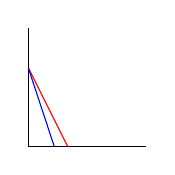
\begin{tikzpicture}
\draw (0,0) -- (1.5,0);
\draw (0,0) -- (0,1.5);
\draw[red] (0,1) -- (0.5,0);
\draw[blue] (0,1) -- (0.33,0);
\end{tikzpicture}

If
\begin{equation*}
\begin{aligned}
f\left(x\right) = \left\{\begin{array}{ll}
1 & x=0\\
0 & x>0
\end{array}
\right.
\end{aligned}
\end{equation*}
then $\left(f_n\right) \to f$ pointwise. Then $\left(f_n\right)$ is bounded with respect to $||\cdot||_\infty$ but has no convergent subsequence.
\begin{proof}
Suppose $\left(f_{n_j}\right) \to g$ uniformly, then $\left(f_{n_j}\right) \to g$ pointwise, so $g=f$. But $f \not\in C\left[0,1\right]$, so $\left(f_{n_j}\right) \not\to f$ uniformly.
\end{proof}
\end{eg}

\begin{defi}
We say $A \subset V$ is sequentially compact (s.compact) if any sequence $\left(\mathbf{v}_n\right)$ in $A$ has a convergent subsequence $\left(\mathbf{v}_{n_j}\right) \to \mathbf{v} \in A$.
\end{defi}

\begin{eg}
$R$ is not s.compact, since $\left(n\right)$ has no convergent subsequence.
\end{eg}

\begin{eg}
$A=\left(0,2\right)$ is not s.compact, since $\left(\frac{1}{n}\right) \to 0 \not\in A$.
\end{eg}

\begin{prop}
Suppose $A \subset V$ is s.compact. Then $A$ is closed in $V$ and bounded.
\begin{proof}
We prove the contrapositive:

If $A$ is not closed, then there exists a sequence $\left(\mathbf{v}_n\right) \to \mathbf{v}$ with $\mathbf{v}_n \in A$ for all $n$ but $\mathbf{v} \not\in A$. By the exercise, any subsequence $\left(\mathbf{v}_{n_j}\right)$ converges to $\mathbf{v} \not\in A$. So $A$ is not s.compact.

If $A$ is not bounded, then for all $n \in \N$ we can find $\mathbf{v}_n \in A$ with $||\mathbf{v}_n|| \geq n$. We claim that $\left(\mathbf{v}_{n_j}\right)$ has no convergent subsequence: if $\left(\mathbf{v}_{n_j}\right) \to \mathbf{v}$, then $\exists J$ s.t. $||\mathbf{v}_{n_j} - \mathbf{v}|| < 1$ for all $j > J$. So
\begin{equation*}
\begin{aligned}
||v_{n_j}|| \leq ||\mathbf{v}|| + ||\mathbf{v_{n_j}} - \mathbf{v}|| \leq ||\mathbf{v}|| + 1
\end{aligned}
\end{equation*}
for all $j>J$, but this is impossible since $n_j\geq j$, so $||v_{n_j}|| \geq j \to \infty$ as $j \to \infty$.

It follows that $\mathbf{v}_n$ has no convergent subsequence, so $A$ is not s.compact.
\end{proof}
\end{prop}

\begin{thm} (Heine-Borel) $A \subset \R^n$ is s.compact if and only if $A$ is closed and bounded.
\begin{proof}
By the proposition, $A$ is s.compact $\implies$ $A$ is closed and bounded.\\
Conversely, suppose $A$ is closed and bounded, and $\left(\mathbf{v}_n\right)$ is a sequence in $A$. Then $\left(\mathbf{v}_n\right)$ is bounded (since $A$ is). So by B-W, it has a convergent subsequence. Since $A$ is closed, $\mathbf{v} \in A$. So $A$ is s.compact.
\end{proof}
\end{thm}

\begin{rem}
By previous example, $\bar{B}_1\left(0\right)$ in $C\left[0,1\right]$ with $||\cdot||_\infty$ is closed and bounded but not s.compact since $\left(f_n\right)$ has no convergent subsequence. So Heine-Borel theorem does not hold in general spaces.
\end{rem}

\begin{rem} If $A \subset V$ a normed space, then $A$ is s.compact $\iff$ $A$ is compact.
\end{rem}

\begin{prop}
Suppose $C \subset V$ is s.compact and $f:C\to W$ is continuous. Then $f\left(C\right)$ is s.compact.
\begin{proof}
Suppose $\left(\mathbf{w}_n\right)$ is a sequence in $f\left(C\right)$. Pick $\mathbf{v}_n \in C$ with $f\left(\mathbf{v}n\right) = \mathbf{w}_n$. We know $C$ is s.compact, so $\left(\mathbf{v}_n\right)$ has a convergent subsequence $\left(\mathbf{v}_{n_j}\right) \to \mathbf{v} \in C$.

Now $f$ is continuous, so $\left(\mathbf{w}_{n_j}\right) = \left(f\left(\mathbf{v}_{n_j}\right)\right) \to \left(f\left(\mathbf{v}\right)\right) \in f\left(C\right)$. So $f\left(C\right)$ is s.compact.
\end{proof}
\end{prop}

We'll use the above to prove maximum value theorem.

\begin{lemma}
If $A \subset \R$ is closed and bounded, then $\sup A\in A$.
\begin{proof}
$A$ is bounded, so $\sup A$ exists. Pick $x_n \in A$ with $\sup A - \frac{1}{n} \leq x_n \leq \sup A$. Then $\left(x_n\right) \to \sup A$. The result follows since $A$ is closed.
\end{proof}
\end{lemma}

\begin{thm} (Maximum value theorem) Suppose $C$ is s.compact, $f:C\to \R$ is continuous. Then there exists $\mathbf{v} \in V$ s.t.
\begin{equation*}
\begin{aligned}
f\left(\mathbf{v}\right) \geq f\left(\mathbf{v'}\right)
\end{aligned}
\end{equation*}
for all $\mathbf{v'} \in C$.
\begin{proof}
We know $A = f\left(C\right)$ is a s.compact subset of $\R$, so it is closed and bounded. So by the lemma, $\sup A$ is in $A = f\left(C\right)$. So pick $\mathbf{v}\in C$ with $f\left(\mathbf{v}\right) = \sup A$.
\end{proof}
\end{thm}

Application: Norms on $\R^n$:

Let $||\cdot||$ be a norm on $\R^n$.

\begin{lemma}
The map id:$\left(\R^n,||\cdot||_1\right) \to \left(\R^n,||\cdot||\right)$ is continuous.
\begin{proof}
Write $\mathbf{v} = \left(v_1,...,v_n\right) = \sum_{i=1}^n v_i \mathbf{e}_i$. By the triangle inequality,
\begin{equation*}
\begin{aligned}
||\mathbf{v}|| \leq \sum_{i=1}^n ||v_i\mathbf{e}_i|| = \sum_{i=1}^n |v_i| ||\mathbf{e}_i|| \leq C \sum_{i=1}^n |v_i| = C||\mathbf{v}||_1
\end{aligned}
\end{equation*}
Where $C = \max_{1\leq i} \leq n\left\{||\mathbf{e}_j||\right\}$. By criterion of section 1.4, the given map is continuous.
\end{proof}
\end{lemma}

\begin{coro}
The map $f:\left(\R^n, ||\cdot||_1\right) \to \R$ given by $f\left(\mathbf{v}\right) = ||\mathbf{v}||$ is continuous.
\end{coro}

\begin{thm}
$||\cdot||$ is Lipschitz equivalent to $||\cdot||_1$.
\begin{proof}
Let $S = \left\{\mathbf{v}\in\R^n \mid ||\mathbf{v}_1 = 1\right\} = g^{-1}\left(\left\{1\right\}\right)$, where $g\left(\mathbf{v}\right) = ||\mathbf{v}||_1$.

Now $g:\left(\R^n,||\cdot||_1\right) \to \R$ is continuous, $\left\{1\right\}$ is closed in $\R$, so $g^{-1}\left(\left\{1\right\}\right)$ is closed in $\left(\R^n,||\cdot||_1\right)$. $S$ is also obviously bounded in $\left(\R^n,||\cdot||_1\right)$. So $S$ is s.compact by Heine-Borel.

$f:\left(\R^n,||\cdot||_1\right) \to \R$, $f\left(\mathbf{v}\right) = ||\mathbf{v}||$ is continuous by corollary. So by maximum value theorem, there exists $\mathbf{v_\pm} \in S$ s.t.
\begin{equation*}
\begin{aligned}
C_- = f\left(\mathbf{v}_-\right) \leq f\left(\mathbf{v}\right) \leq f\left(\mathbf{v}_+\right) = C_+
\end{aligned}
\end{equation*}
for all $\mathbf{v} \in S$, i.e. $C_- \leq \mathbf{v} \leq \C_+$ for all $\mathbf{v} \in S$ where $C_- = ||\mathbf{v}_-||>0$ since $\mathbf{v}_- \in S \implies \mathbf{v_-} \neq \mathbf{0} \implies \mathbf{v_-} \neq 0$.

Then for $\mathbf{v} \neq 0$ in $\R^n$, $\mathbf{v}/||\mathbf{v}||_1 \in S$. So
\begin{equation*}
\begin{aligned}
0 < C_- \leq ||\frac{\mathbf{v}}{||\mathbf{v}||_1} \leq C_+
\end{aligned}
\end{equation*}
i.e.
\begin{equation*}
\begin{aligned}
C_-||\mathbf{v}||_1 \leq ||\mathbf{v}|| \leq C_+ ||\mathbf{v}||_1
\end{aligned}
\end{equation*}
where $C_-,C_+ > 0$. So the two norms are Lipschitz equivalent.
\end{proof}
\end{thm}

\begin{coro}
Any two norms on $\R^n$ are Lipschitz equivalent.
\end{coro}

\subsection{Completeness}
Let $V$ be a normed space, and let $\left(\mathbf{v}_n\right)$ be a sequence in $V$.

\begin{defi}
The sequence $\left(\mathbf{v}\right)_n$ is \emph{Cauchy} if given $\varepsilon > 0$, there exists $N$ s.t. $||\mathbf{v}_n - \mathbf{v}_m|| < \varepsilon$ for all $n,m \geq N$.
\end{defi}

\begin{eg}
If $\left(\mathbf{v}_n\right) \to \mathbf{v}$, then $\left(\mathbf{v}_n\right)$ is Cauchy.
\begin{proof}
Given $\varepsilon>0$, pick $N$ s.t. $||\mathbf{v}_n-\mathbf{v}|| < \frac{\varepsilon}{2}$ for all $n \geq N$. Then for $n,m \geq N$, by triangle inequality,
\begin{equation*}
\begin{aligned}
||\mathbf{v}_n - \mathbf{v}_m|| \leq ||\mathbf{v}_n - \mathbf{v}||+||\mathbf{v}-\mathbf{v}_m|| < \varepsilon
\end{aligned}
\end{equation*}
i.e. $\left(\mathbf{v}_n\right)$ is Cauchy.
\end{proof}
\end{eg}

\begin{eg}
Let $s_n = \sum_{i=1}^n \frac{1}{i}$. Then $s_n$ diverges. Also it is not Cauchy, even though $|s_n - s_{n+1}| \to 0$ as $n \to \infty$.
\end{eg}

Cauchy sequences \emph{want} to converge.

\begin{eg}
Given $\varepsilon>0$, pick $N$ s.t. $||\mathbf{v}_n - \mathbf{v}_m|| < \varepsilon$ for all $n,m \geq N$. Then all but finitely many terms of $\left(\mathbf{v}_n\right)$ are contained in $B_\varepsilon\left(\mathbf{v}_N\right)$.
\end{eg}

However they may not have an element of $V$ to converge to.

\begin{eg}
Let $V=C\left[0,1\right]$ with $||\cdot||_1$. Take
\begin{equation*}
\begin{aligned}
f_n = \left\{\begin{array}{ll}
0 & x\in\left[0,1/2\right]\\
n\left(x-1/2\right) & x\in\left[1/2,1/2+1/n\right]\\
1 & x \in \left[1/2+1/n,1\right]
\end{array}
\right.
\end{aligned}
\end{equation*}

\begin{tikzpicture}
\begin{axis}[xmin=0,xmax=1.5,ymin=0,ymax=1.5]
\addplot coordinates {
	(0,0)
	(0.5,0)
	(0.6,1)
	(1,1)
};
\end{axis}
\end{tikzpicture}

$f\left(n\right)$ is Cauchy:\\
If $m,n \geq >N$, $|f_n\left(x\right) - f_m\left(x\right)| = 0$ if $x \not\in A_n = \left[1/2,1/2+1/N\right]$, and $<1$ if $x \in A_N$. Then
\begin{equation*}
\begin{aligned}
||f_n - f_m||_1 = \int_0^1 |f_n\left(x\right) - f_m\left(x\right)| dx \leq \int_{1/2}^{1/2+1/N} 1 dx = \frac{1}{N}
\end{aligned}
\end{equation*}

so $\left(f_n\right)$ is Cauchy.

Now let $$f\left(x\right) = \left\{\begin{array}{ll}
0 & x\in\left[0,1/2\right]\\
1 & x\in\left(1/2,1\right]
\end{array}
\right.$$
which is not in $C\left[0,1\right]$.

If $\left(f_n\right) \to g \in C\left[0,1\right]$ then $\left(f_n\right) \to g$ with respect to $||\cdot||_1$ on $\left[0,1\right] - A_n$ for any $N>0$. On the other hand, $\left(f_n\right) \to f$ uniformly on $\left[0,1\right]-A_N$ for any $N>0$.

On the other hand, $\left(f_n\right) \to f$ uniformly on $\left[0,1\right] - A_N$ for any $N>0$. So $\left(f_n\right) \to f$ with respect to $||\cdot||_1$ on $\left[0,1\right]-A_N$ for all $N>0$. Therefore $g\left(x\right) = f\left(x\right)$ for all $x \in \left[0,1\right]$. Contradiction.
\end{eg}

\begin{defi}
A normed space $V$ is \emph{complete} if every Cauchy sequence $\left(\mathbf{v}_n\right)$ in $V$ converges to a limit $\mathbf{v} \in V$.
\end{defi}

\begin{eg}
$\left(C\left[0,1\right],||\cdot||_1\right)$ is not complete.
\end{eg}

Application: Completeness of $\R^n$.

Let $V$ be a normed vector space, and suppose $\left(\mathbf{v}_n\right)$ is a Cauchy sequence in $V$.

\begin{lemma}
$\left(\mathbf{v}_n\right)$ is bounded. (Exercise)
\end{lemma}

\begin{lemma}
If $\left(\mathbf{v}_n\right)$ has a convergent subsequence $\left(\mathbf{v}_{n_i}\right) \to \mathbf{v} \in V$, then $\left(\mathbf{v}_n\right) \to \mathbf{v}$.
\begin{proof}
Given $\varepsilon>0$, pick $M$ s.t. $||\mathbf{v}_n - \mathbf{v}_m|| < \frac{\varepsilon}{2}$ whenever $n,m > M$. Now $\mathbf{v}_{n_i}$ converges to $\mathbf{v}$, so pick $I$ s.t. $||\mathbf{v}_{n_i}-\mathbf{v}|| < \frac{\varepsilon}{2}$ whenever $i>I$.\\
So choose $I'>I$ s.t. $n_{I'} \geq M$. Then for $n>n_{I'}$,
\begin{equation*}
\begin{aligned}
||\mathbf{v}_n - \mathbf{v}|| \leq ||\mathbf{v}_n - \mathbf{v}_{n_{I'}}|| + ||\mathbf{v}_{n_{I'}} - \mathbf{v}|| < \varepsilon
\end{aligned}
\end{equation*}
So $\left(\mathbf{v}_n\right) \to \mathbf{v}$.
\end{proof}
\end{lemma}

\begin{thm}
$\R^n$ is complete.
\begin{proof}
Suppose $\left(\mathbf{v}_n\right)$ is a Cauchy sequence in $\R^n$. By lemma 1, $\left(\mathbf{v}_n\right)$ is bounded. By B-W, $\left(\mathbf{v}_n\right)$ has a convergent subsequence $\left(\mathbf{v}_{n_i}\right)\to \mathbf{v}$. By lemma 2, $\left(\mathbf{v}_n\right) \to \mathbf{v}$, i.e. every Cauchy sequence converges. So $\R^n$ is complete.
\end{proof}
\end{thm}

\begin{rem}
If $||\cdot||$ and $||\cdot||'$ are Lipschitz equivalent, then $\left(\mathbf{v}_n\right)$ is Cauchy with respect to the two norms are equivalent. So Completeness with respect to the two norms are equivalent.

Since all norms on $\R^n$ are Lipschitz equivalent, the the theorem holds for any norm. 

We saw $\left(C\left[0,1\right],||\cdot||_1\right)$ is not complete. What about $\left(C\left[0,1\right],||\cdot||_\infty\right)$?

Bounded sequences need not have convergent subsequences.
\end{rem}

\begin{thm}
$C\left[0,1\right]$ is complete with respect to $||\cdot||_\infty$.
\begin{proof}
Given a Cauchy sequence $\left(f_n\right)$, we must find $f\in C\left[0,1\right]$ s.t. $\left(f_n\right) \to f$ uniformly.

Given $\varepsilon>0$, choose $N$ s.t. $||f_n-f_m||<\varepsilon/2$ for all $n,m \geq N.$ Then if $x \in \left[0,1\right]$,
\begin{equation*}
\begin{aligned}
|f_n\left(x\right) - f_m\left(x\right) &\leq \max_{x \in \left[0,1\right]} |f_n\left(x\right) - f_m\left(x\right)|\\
&= ||f_n-f_m||_\infty\\
&<\varepsilon/2 < \varepsilon
\end{aligned}
\end{equation*}
For $n,m \geq N$.

So $\left(f_n\left(x\right)\right)$ is a Cauchy sequence in $\R$. But $\R$ is complete. So $\lim_{n \to \infty} f_n\left(x\right)$ exists.

Define $f\left(x\right) = \lim_{n\to\infty} f_n\left(x\right)$. Then $\left(f_n\right) \to f$ pointwise.

Now we want to prove $\left(f_n\right) \to f$ uniformly. Given $\varepsilon>0$, and $x \in \left[0,1\right]$, pick $M$ (depending on $x$) s.t. $|f_n\left(x\right)-f\left(x\right) < \varepsilon/2$ whenever $n\geq M$.

Let $R = \max\left(N,M\right)$, then for $n\geq N$,
\begin{equation*}
\begin{aligned}
|f_n\left(x\right) - f\left(x\right)| &\leq |f_n\left(x\right)-f_R\left(x\right)| + |f_R\left(x\right) - f\left(x\right)|\\
&< \varepsilon/2 + \varepsilon/2 = \varepsilon
\end{aligned}
\end{equation*}
for $n,R \geq N$.
i.e. $|f_n\left(x\right) - f\left(x\right)| < \varepsilon$ for all $x \in \left[0,1\right]$ i.e. $||f_n-f||_\infty < \varepsilon$.\\
So $\left(f_n\right) \to f$ uniformly.

$f_n\in C\left[0,1\right] \implies f\in C\left[0,1\right]$. So $\left(f_n\right) \to f\in C\left[0,1\right]$ uniformly.
\end{proof}
\end{thm}

\subsection{Uniform continuity}
Suppose $V,W$ are normed spaces, $A \subset V$.

\begin{defi}
$f:A \to W$ is \emph{uniformly continuous} if for every $\varepsilon>0$, $\exists \delta > 0$ s.t. $||f\left(\mathbf{v}\right) - f\left(\mathbf{v}'\right) || < \varepsilon$ whenever $||\mathbf{v}-\mathbf{v}'||<\delta$.
\end{defi}

\begin{eg}
Let $f:\R \to \R$ by $f\left(x\right) = x^2$. Then $f\left(x+\delta\right) - f\left(x\right) = 2x\delta + \delta^2$. For fixed $\delta$, $2x\delta+\delta^2 \to \infty$ as $x \to \infty$. So $f\left(x\right) =x^2$ is not uniformly continuous.
\end{eg}

\begin{eg}
Let $f:\left(0,1\right] \to \R$ with $f\left(x\right) = \frac{1}{x}$. This is not uniformly continuous as well (consider $x \to 0$).
\end{eg}

\begin{thm}
If $C$ is s.compact, and $f:C \to W$ is continuous, then $f$ is uniformly continuous.
\begin{proof}
Suppose $f$ is not uniformly continuous. Then there exists $\varepsilon>0$ s.t. for all $n>0$ we can find $\mathbf{v}_n,\mathbf{w}_n\in C$ with $||\mathbf{v}_n-\mathbf{w}_n|| < \frac{1}{n}$, and $||f\left(\mathbf{v}_n\right)-f\left(\mathbf{w}_n\right)|| \geq \varepsilon$ (else $f$ is uniformly continuous).

Since $C$ is s.compact, $\left(\mathbf{v}_n\right)$ has a convergent subsequence $\left(\mathbf{v}_{n_i}\right) \to \mathbf{v^*} \in C$.

$f$ is continuous and $\mathbf{v}^* \in C$, so $\exists \delta > 0$ s.t. $||f\left(\mathbf{v}\right)-f\left(\mathbf{v^*}\right)|| < \varepsilon/2$ whenever $\mathbf{v}\in B_\delta\left(\mathbf{v^*}\right)$.

If $\mathbf{v},\mathbf{v'} \in B_\delta\left(\mathbf{v^*}\right)$, then
\begin{equation*}
\begin{aligned}
||f\left(\mathbf{v}\right) - f\left(\mathbf{v}'\right) || &\leq ||f\left(\mathbf{v}\right)-f\left(\mathbf{v}^*\right)|| + ||f\left(\mathbf{v}^*\right)-f\left(\mathbf{v}'\right)||\\ &< \varepsilon/2+\varepsilon/2 = \varepsilon
\end{aligned}
\end{equation*}
$\left(\mathbf{v}_{n_i}\right) \to \mathbf{v}^*$, so pick $I_1$ s.t. $||\mathbf{v}_{n_i} - \mathbf{v}^*|| < \delta/2$ when $i \geq I_1$.

Pick $I_2$ s.t. $1/I_2 < \delta/2$. Then for $i \geq \max\left(I_1,I_2\right)$, we have $||\mathbf{v}_{n_i} - \mathbf{v}^*|| < \delta/2$ and $||\mathbf{v}_{n_i} - \mathbf{w}_{n_i} || < \frac{1}{n_i} < \frac{1}{i} < \frac{1}{I_2} < \frac{\delta}{2}$.

So $||\mathbf{w}_{n_i} - \mathbf{v}^*|| < ||\mathbf{w}_{n_i} - \mathbf{v}_{n_i}|| + ||\mathbf{v}_{n_i} - \mathbf{v}^*|| < \delta/2+\delta/2 = \delta$, i.e. $\mathbf{w}_{n_i},\mathbf{v}_{n_i} \in B_\delta \left(\mathbf{v}^*\right)$, $||f\left(\mathbf{v}_{n_i}\right) - f\left(\mathbf{w}_{n_i}\right)|| \geq \varepsilon$. Contradiction. So $f$ must be uniformly continuous.
\end{proof}
\end{thm}

\subsection{Application: Integration}
Recall from Analysis I:
We say $f: \left[a,b\right] \to \R$ is piecewise constant if $\exists a=a_0<a_1<...<a_n=b$ and $c_1,...,c_n \in \R$ s.t. $f\left(x\right) = c_i$ if $x\in \left(a_{i-1},a_i\right)$.

\begin{tikzpicture}
\begin{axis}[xmin=0,xmax=1.5,ymin=0,ymax=1.5]
\addplot coordinates {
	(0.2,0.5) (0.5,0.5)
	
	(0.5,1) (1,1)
	
	(1,0.2) (1.2,0.2)
};
\end{axis}
\end{tikzpicture}

Let $P\left[a,b\right] = \left\{ f:\left[a,b\right] \to \R \mid f \text{ is piecewise constant} \right\}$. If $f \in P\left[a,b\right]$ is as above, then
\begin{equation*}
\begin{aligned}
I\left(f\right) = \sum_{i=1}^n c_i \left(a_i - a_{i-1}\right) = "\int" f
\end{aligned}
\end{equation*}

\begin{lemma}
If $f,g \in P\left[a,b\right]$, $\lambda \in \R$, then
\begin{equation*}
\begin{aligned}
f-\lambda g \in P\left[a,b\right]
\end{aligned}
\end{equation*}
and $I\left(f-\lambda g\right) = I\left(f\right) - \lambda I\left(g\right)$.
\end{lemma}

Write $f\geq g$ if $f\left(x\right) \geq g\left(x\right)$ for all $x\in\left[a,b\right]$.

\begin{lemma}
If $f\geq 0$, $I\left(f\right) \geq 0$.
\end{lemma}

So if $f,g\in P\left[a,b\right], f\geq g$, then $I\left(f\right) \geq I\left(g\right)$.

\begin{defi} (Riemann Integral) Suppose $f:\left[a,b\right] \to \R$ is bounded. Let
\begin{equation*}
\begin{aligned}
\mathcal{U}\left(f\right) = \left\{ g\in P\left[a,b\right] \mid g\geq f\right\},\\
\mathcal{L}\left(f\right) = \left\{ g\in P\left[a,b\right] \mid g\leq f\right\}
\end{aligned}
\end{equation*}
since $f$ is bounded, these are not empty.\\
Let 
\begin{equation*}
\begin{aligned}
U\left(f\right) = \left\{I\left(g\right) \mid g \in \mathcal{U}\left(f\right)\right\},\\
L\left(f\right) = \left\{I\left(g\right) \mid g \in \mathcal{L}\left(f\right)\right\}
\end{aligned}
\end{equation*}

If $g^+ \in \mathcal{U}\left(f\right)$ and $g^- \in \mathcal{L}\left(f\right)$, then $g^+ \geq f \geq g^-$. So $I\left(g^+\right) \geq I\left(g^-\right)$. If $u \in U\left(f\right)$ and $l \in L\left(f\right)$, then $u \geq l$. So $U\left(f\right)$ is bounded below, $L\left(f\right)$ is bounded above.

Now let 
\begin{equation*}
\begin{aligned}
u\left(f\right) = \inf U\left(f\right),\\
l\left(f\right) = \inf L\left(f\right)
\end{aligned}
\end{equation*}

Note that $u\left(f\right) \geq l\left(f\right)$.

We say $f$ is Riemann integrable if $u\left(f\right) = l\left(f\right)$, in which case we define 
\begin{equation*}
\begin{aligned}
\int_a^b f\left(x\right) dx = u\left(f\right) = l\left(f\right)
\end{aligned}
\end{equation*}
\end{defi}

If $f \in P\left[a,b\right]$, then $u\left(f\right) = I\left(f\right) = l\left(f\right)$, so $f$ is RI.

\begin{thm}
If $f\in C\left[a,b\right]$, then $f$ is RI.
\end{thm}

\begin{lemma}
Given $\varepsilon>0$, $\exists g^+ \in \mathcal{U}\left(f\right)$ and $g^- \in \mathcal{L}\left(f\right)$ s.t. $I\left(g^+\right) - I\left(g^-\right) < \varepsilon$.
\begin{proof}
$\left[a,b\right]$ is closed and bounded in $\R$, so it is s.compact. By last lecture's theorem, $f: \left[a,b\right] \to \R$ is uniformly continuous.\\
So pick $\delta$ s.t.
\begin{equation*}
\begin{aligned}
|f\left(x\right) - f\left(y\right) | < \frac{\varepsilon}{b-a}
\end{aligned}
\end{equation*}
whenever $|x-y| < \delta$. Choose $a=a_0<a_1<...<a_n = b$ such that $a_{i+1}-a_i < \delta$ for all $i$.

Define
\begin{equation*}
\begin{aligned}
c_i^+ = \max_{x\in\left[a_{i-1},a_i\right]} f\left(x\right),\\
c_i^- = \min_{x\in\left[a_{i-1},a_i\right]} f\left(x\right)
\end{aligned}
\end{equation*}
(These exist by Maximum value theorem) So 
\begin{equation*}
\begin{aligned}
c_i^+ = f\left(x^+\right) \geq f\left(x^-\right) \forall x \in \left[a_{i-1},a_i\right],\\
c_i^- = f\left(x^-\right) \leq f\left(x\right) \forall x\in\left[a_{i-1},a_i\right]
\end{aligned}
\end{equation*}
$x^+,x^- \in \left[a_{i-1},a_i\right] \implies |x^+ - x^-| < \delta$.

Define 
\begin{equation*}
\begin{aligned}
g^+\left(x\right) = c_i^+ \text{ if } x \in \left[a_{i-1},a_i\right),\\
g^-\left(x\right) = c_i^- \text{ if } x \in \left[a_{i-1},a_i\right)
\end{aligned}
\end{equation*}
Then $|x^+ - x^-| < \delta \implies c_i^+ - c_i^- < \frac{\varepsilon}{b-a}$ for all $i$. So to sum up, $g^+ \geq f \geq g^-$ and $g^+ - g^- \leq \frac{\varepsilon}{b-a}$.\\
Thus $g^+ \in \mathcal{U}\left(f\right)$, $g^- \in \mathcal{L}\left(f\right)$, and 
\begin{equation*}
\begin{aligned}
I\left(g^+\right) - I\left(g^-\right) = I\left(g^+-g^-\right) \leq I\left(\frac{\varepsilon}{b-a}\right) = \varepsilon
\end{aligned}
\end{equation*}
\end{proof}
\end{lemma}

Now prove the theorem:
\begin{proof}
$I\left(g^+\right) \geq u\left(f\right) \geq l\left(f\right) \geq I\left(g^-\right)$. So $u\left(f\right) - l\left(f\right) \leq I\left(g^+\right) - I\left(g^-\right) < \varepsilon$ for all $\varepsilon>0$, which implies $u\left(f\right) = l\left(f\right)$.
\end{proof}

\begin{coro}
If $f \in C\left[a,b\right]$, $\exists f_k \in P\left(a,b\right)$ s.t. $\left(f_k\right) \to f$ uniformly on $\left[a,b\right]$.
\begin{proof}
For each $k$, choose $g_k^+$ as in the proof of lemma with $\varepsilon = \frac{1}{k}$. Then $\left(g_k^+\right) \to f$ uniformly.
\end{proof}
\end{coro}

\begin{eg}(Speed and Distance)
Suppose $f\left[a,b\right] \to \R^n$ is continuous. $f\left(t\right) = \left(f_1\left(t\right),...,f_n\left(t\right)\right)$ where all $f_i$ are continuous.\\
Define $\int_a^b f\left(t\right) dt = \left(f_1\left(t\right) dt, ..., \int_a^b f_n\left(t\right) dt\right)$ (Integrating pointwise).

If $f\left(t\right) = \mathbf{v}\left(t\right) = $velocity of a particle in $\R^n$ at time $t$, then $\mathbf{p}\left(b\right) - \mathbf{p}\left(a\right) = \int_a^b f\left(t\right) dt$ is the displacement of particle from its position at $t=a$. $||\mathbf{v}\left(t\right)||$ is the speed of particle.
\end{eg}

\begin{prop}
If $f: \left[a,b\right] \to \R^n$ is continuous, then
\begin{equation*}
\begin{aligned}
||\int_a^b f\left(t\right) dt|| \leq \int_a^b ||f\left(t\right)|| dt
\end{aligned}
\end{equation*}
\end{prop}

\begin{lemma}
If $x_i,y_i \in \R$ satisfy:\\
(1) $x_i \leq y_i$ for all $i$;\\
(2) $\left(x_i\right) \to x$ and $\left(y_i\right) \to y$\\
Then $x \leq y$.
\begin{proof}
$y_i - x_i \geq 0, \left(y_i-x_i\right) \to y-x \implies y-x\geq 0$.
\end{proof}
\end{lemma}

\begin{lemma}
The proposition holds if $f$ is piecewise constant (maybe not continuous).
\begin{proof}
Suppose $f\left(t\right) = \mathbf{v}_i$ for $t\in\left(a_{i-1},a_i\right)$. Then
\begin{equation*}
\begin{aligned}
||\int_a^b f\left(t\right) dt || &= ||I\left(f\right)||\\
&= ||\sum_{i=1}^n \left(a_{i+1}-a_i\right)\mathbf{v}_i||\\
&\leq \sum_{i=1}^n \left(a_i-a_{i-1}\right) ||\mathbf{v}_i||\\
&= I\left(||f||\right)\\
&= \int_a^b ||f|| dt.
\end{aligned}
\end{equation*}
\end{proof}
\end{lemma}

Proof of proposition:
\begin{proof}
Choose a sequence of piecewise constant functions $f_k: \left[a,b\right] \to \R^n$ s.t. $\left(f_k\right) \to f$ uniformly.\\
Then
\begin{equation*}
\begin{aligned}
\int_a^b f_k \to \int_a^b f
\end{aligned}
\end{equation*}
(uniformly convergence $\implies$ $L^1$ convergence) and
\begin{equation*}
\begin{aligned}
\left(\left|\left|\int_a^b f_k\right|\right|\right) \to \left(\left|\left|\int_a^b f\right|\right| \right)
\end{aligned}
\end{equation*}
since $||\cdot||$ is continuous.

Also $\left(||\mathbf{f}_k||\right) \to ||f||$ uniformly ($||\cdot||$ is continuous). So
\begin{equation*}
\begin{aligned}
\left(\int_a^b ||f_k||\right) \to \int_a^b ||f||
\end{aligned}
\end{equation*}

So now take $x_k = ||\int_a^b f_k||, x=||\int_a^b f||, y_k = \int_a^b ||f_k||, y=\int_a^b ||f||$.

Then $x_k \leq y_k$, so $x \leq y$.
\end{proof}

\newpage

\section{Differentiation}
Slogan: \emph{The derivative is a linear map}.

\subsection{Derivative}
\begin{defi}
Let $U\subset \R^n$ be open, $f:U-\left\{x_0\right\}\to \R^m$. We say
\begin{equation*}
\begin{aligned}
\lim_{x\to x_0} f\left(x\right)=y
\end{aligned}
\end{equation*}
if the function $\bar{f}:U \to \R^m$ given by
\begin{equation*}
\begin{aligned}
\bar{f}\left(x\right) = \left\{\begin{array}{ll}
f\left(x\right) & x \neq x_0\\
y & x=x_0
\end{array}\right.
\end{aligned}
\end{equation*}
is continuous at $x_0$.

Note that we don't care which norms on $\R^n$ or $\R^m$ we use: all the norms on $\R^n$ are Lipschitz equivalent, so they determine the same continuous functions.
\end{defi}

\begin{defi}
Suppose $U \subset \R^n$ is open, $x_0 \in U$ and $f:U\to \R^m$. We say $f$ is differentiable at $x_0$ if there is a linear map $L:\R^n \to \R^m$ s.t.
\begin{equation*}
\begin{aligned}
\lim_{v\to 0} \frac{f\left(x_0+v\right)-(f(x_0)+L(v))}{||v||} = 0
\end{aligned}
\end{equation*}
\end{defi}

If such an $L$ exists, it is unique.
\begin{proof}
Suppose $L_1,L_2$ exist. Subtracting the two limit equations gives
\begin{equation*}
\begin{aligned}
\lim_{v \to 0} \frac{L_2(v)-L_1(v)}{||v||} = 0
\end{aligned}
\end{equation*}
If $v \in \R^n$, $v\neq 0$, then $tv \to 0$ as $t\to 0^+$. So
\begin{equation*}
\begin{aligned}
\lim_{t\to 0^+} \frac{L_2(tv)-L_1(tv)}{||tv||} = 0
\end{aligned}
\end{equation*}
Since $L_1,L_2$ are linear maps, simplify that and we get $L_2(v)=L_1(v)$. But $v$ is arbitrary. So $L_1=L_2$.
\end{proof}

When the equation in the definition of differentiability holds, we say
\begin{equation*}
\begin{aligned}
Df|_{x_0} = L
\end{aligned}
\end{equation*}
is the \emph{derivative} of $f$ at $x_0$. Note that $Df|_{x_0}$ is a \emph{linear map} from $\R^n$ to $\R^m$.

Equivalently, $f$ is differentiable at $x_0$ with $Df|_{x_0}=L$ if 
\begin{equation*}
\begin{aligned}
f(x_0+v)=f(x_0)+L(v)+||v||\alpha(v)
\end{aligned}
\end{equation*}
where $\lim_{v\to 0} \alpha(v) = 0$.

\begin{prop}
Suppose $f:U\to \R^m$ is differentiable at $x_0 \in U$. Then $f$ is continuous at $x_0$.
\end{prop}

\begin{lemma}
Suppose $L:\R^n \to (W,||\cdot||)$ is a linear map where $W$ is a normed space. Then $\lim_{v \to 0} L(v) = 0$.
\end{lemma}

Note that the lemma is false if $\R^n$ is replaced by an arbitrary normed space.

\begin{proof}
Let $v=(v_1,...,v_n) = \sum_{i=1}^n v_i e_i$. Then
\begin{equation*}
\begin{aligned}
||L(v)||&=||\sum_{i=1}^n v_i L(e_i)||\\
&\leq \sum_{i=1}^n |v_i| \cdot ||L(e_i)||\\
&\leq C\sum_{i=1}^n |v_i| \\
&= C||v||_1
\end{aligned}
\end{equation*}
Where $C=\max \{||L(e_1)||,...,||L(e_n)||\}$.

Given $\varepsilon>0$, pick $\delta > \varepsilon/C$. If $||v||_1 < \delta$ then $||L(v)||<\varepsilon$, so $\lim_{v\to 0}L(v) = 0$.
\end{proof}

Prove of proposition:
\begin{proof}
Since $f$ is differentiable at $x_0$, we have
\begin{equation*}
\begin{aligned}
f(x_0+v) = f(x_0)+L(v)+||v||\alpha(v)
\end{aligned}
\end{equation*}
where $\lim_{v\to 0} \alpha(v) = 0$. Now take the limit $v \to 0$ of both sides we have
\begin{equation*}
\begin{aligned}
\lim_{v\to 0} f(x_0+v) = f(x_0)
\end{aligned}
\end{equation*}
So $f$ is continuous at $x_0$.
\end{proof}

\subsection{The derivative as a matrix}
Suppose $U \subset \R^n$ is open, $f:U \to \R^m$.

We say $f$ is differentiable if $f$ is differentiable at all $x \in U$.

If so, we have $Df:U \to \mathcal{L}(\R^n,\R^m)$.

From Linear Algebra we know that there is a bijection between $\mathcal{L}(\R^n,\R^m)$ and the set of $m\times n$ real matrix:
\begin{equation*}
\begin{aligned}
[a_{ij}] \longleftrightarrow L(e_j) = \sum a_{ij} e_i
\end{aligned}
\end{equation*}

Now let's consider given $f:U \to \R^m$, how we compute $Df=[a_{ij}(x)]$. We first reduce to the case $m=1$ by writing
\begin{equation*}
\begin{aligned}
f(x) = (f_1(x),...,f_n(x))
\end{aligned}
\end{equation*}
Then think about $F:U \to \R$.

\begin{prop}
$f$ is differentiable at $x_0$ if and only if $f_i$ is differentiable for all $1\leq i \leq m$. If so,
\begin{equation*}
\begin{aligned}
Df|_{x_0} = (Df_1|_{x_0},...,Df_m|_{x_0}).
\end{aligned}
\end{equation*}
\begin{proof}
Suppose $g: U \to \R^m$. Using the uniform norm on $\R^m$, we see that $\lim_{v\to 0} g(v) = 0$ iff $\lim_{v \to 0} g_i(v) = 0$ for all $1 \leq i \leq m$.

Now let $L: \R^n \to \R^m$. Then
\begin{equation*}
\begin{aligned}
\lim_{v\to 0} \frac{f(x_0+v)-(f(x_0)+L(v))}{||v||} = 0
\end{aligned}
\end{equation*}
if and only if
\begin{equation*}
\begin{aligned}
\lim_{v\to 0} \frac{f_i(x_0+v)-(f_i(x_0)+L_i(v))}{||v||} = 0
\end{aligned}
\end{equation*}
for all $1 \leq i \leq m$, i.e. $f_i$ is differentiable at $x_0$ and $Df_i|_{x_0} = L_i$.
\end{proof}
\end{prop}

Summary: 
\begin{equation*}
\begin{aligned}
Df|_{x_0} = \left[\begin{array}{ll}
Df_1|_{x_0}\\
...\\
Df_m|_{x_0}
\end{array}\right]
\end{aligned}
\end{equation*}
where $Df_i|_{x_0} : \R^n \to \R$ is a $1 \times n$ matrix $[a_1,...,a_n]$.

\begin{defi} (Directional Derivative)\\
Suppose $F:U\to\R$. If $v \in \R^n$, the \emph{directional derivative} of $F$ in direction $v$ at $x$ is
\begin{equation*}
\begin{aligned}
D_v F|_x &= \lim_{t \to 0} \frac{F(x+tv)-F(x)}{t}\\
&= \frac{d}{dt} (F(x+tv))|_{t=0}
\end{aligned}
\end{equation*}
\end{defi}

$D_v F$ measures the rate of change of $F$ if I walk away from $x$ at velocity $v$.

It's also helpful to consider
\begin{equation*}
\begin{aligned}
D_v^+ F = \lim_{t \to 0^+} \frac{F(x+tv)-F(x)}{t}
\end{aligned}
\end{equation*}
and similarly for $D_v^- F$. We can prove that
\begin{equation*}
\begin{aligned}
D_v^- F|_x = -D_{-v}^+ F|_x
\end{aligned}
\end{equation*}

Note: $D_v F$ exists iff $D_v^+ F, D_v^- F$ both exist and are equal.

\begin{eg}
Consider a special case $v=e_i$. Then
\begin{equation*}
\begin{aligned}
D_i F|_x &= \frac{\partial F}{\partial x_i}|_x\\
&=D_{e_i}F|_x\\
&=\frac{d}{dt} (F(x_1,...,x_i+t,...,x_n))|_{t=0}\\
&= \frac{d}{dt} (F(x_1,...,x_{i-1},t,x_{i+1},...,x_n))|_{t=x}
\end{aligned}
\end{equation*}
is the $i$th partial derivative of $F$.
\end{eg}

\begin{prop}
If $F: U \to \R$ is differentiable at $x$, then $D_v F|_x = DF|_x(v)$.
\begin{proof}
If $v=0$ then both sides are $0$.

If $v \neq 0$, then $tv \to 0$ as $t \to 0^+$, so differentiability of $F$ implies
\begin{equation*}
\begin{aligned}
\lim_{t \to 0^+} \frac{F(x+tv)-((F(x)+L(tv))}{||tv||} = 0
\end{aligned}
\end{equation*}
where $L=DF|_{x}$. So
\begin{equation*}
\begin{aligned}
\lim_{t\to 0^+}\frac{F(x+tv)-F(x)}{t} - L(v) = 0
\end{aligned}
\end{equation*}
i.e. $D_v^+ F|_x = DF|_x(v)$. Then $D_v^-F|_x = -D_{-v}^+ F|_x = -L(-v)=L(v)$.
\end{proof}
\end{prop}

If $DF|_x = [a_1,...,a_n]$ then $a_i = DF|_x(e_i) = D_{e_i} F|_x = D_i F|_x$. So we have
\begin{equation*}
\begin{aligned}
DF|_x = [D_1F|_x,...,D_n F|_x]
\end{aligned}
\end{equation*}

Summary: if $f:\R^n \to \R^m$, then
\begin{equation*}
\begin{aligned}
Df = \left[\begin{array}{ll}
Df_1\\
...\\
Df_m
\end{array}\right]=[D_jf_i]
\end{aligned}
\end{equation*}

\begin{eg}
Let $f:\R^3 \to \R^2$ with $f(x,y,z)=(x^2+y^2+z^2,xyz)$. Then
\begin{equation*}
\begin{aligned}
Df = \left[\begin{matrix}
1 & 2y & 3z^2\\
yz & xz & xy
\end{matrix}\right]
\end{aligned}
\end{equation*}
\end{eg}

Note: Just because $D_i F_x$ all exists doesn't mean that $F$ is differentiable at $x$.

\begin{eg}
Let $F:\R^2 \to \R$ be given by
\begin{equation*}
\begin{aligned}
F(x,y) = \left\{
\begin{array}{ll}
0 & xy=0\\
H(x,y) & \text{ otherwise}
\end{array}\right.
\end{aligned}
\end{equation*}
where $H(x,y)$ is any arbitrary horrible function. Then
\begin{equation*}
\begin{aligned}
D_1F|_0 = D_2F|_0 = 0
\end{aligned}
\end{equation*}
but $F$ may not even be continuous.
\end{eg}

We can even have $D_v F$ well defined for every $v$, but $F$ is not differentiable.
\begin{eg}
Let $S^1 = \{v \in \R^2 | ||v||=1\}$. Choose $h:S  \to \R$ to be any function. Define $F: \R^2 \to \R$ by
\begin{equation*}
\begin{aligned}
F(v)=\left\{\begin{array}{ll}
||v||h(\frac{v}{||v||}) & v \neq 0\\
0 & v = 0
\end{array}\right.
\end{aligned}
\end{equation*}
Then $D_v^+ F|_0 = ||v||h(\frac{v}{||v||})$. If we let $h(-v)=-h(v)$ then $D_v^+ F = D_v^- F$, so $D_v F$ is well defined. Now if $F$ is differentiable, $D_v F|_0 = DF|_0(v)$, so $h(v)$ would have to be a linear function on $S^1$; but $h$ is arbitrary except the one condition above.
\end{eg}

A criterion for differentiability:
Let $U \subset \R^n$ be open.

\begin{defi}
$C^1(U)=\{f:U \to \R|$ for $1 \leq i \leq n$, the partial derivative $D_i f|_x$ exists for all $x \in U$ and is a continuous function of $x\}$.
\end{defi}

\begin{eg}
\begin{equation*}
\begin{aligned}
F(x,y,z) = e^{\cos x^2y+z}-y^2z \in C^1(\R^3)
\end{aligned}
\end{equation*}
\end{eg}

\begin{thm}
If $F \in C^1(U)$, then $F$ is differentiable on $U$.
Tools used in proof:\\
$\bullet$ Alternative characterisation of differentiability in 4.1;\\
$\bullet$ If $\lim_{v\to 0} g(v) = w_0$ and $\lim_{v\to w_0} f(v)=z$, then $\lim_{v \to 0}f(g(v)) = z$;\\
$\bullet$ Suppose $b: U \to \R$ is bounded on $B_r(v_0)$ for some $r>0$. Then $\lim_{v \to v_0} b(v)\alpha(v)=0$ if $\lim_{v\to v_0} \alpha(v) = 0$.
\begin{proof} (of the bullet point):\\
Since $b$ is bounded, there exists $M \in \R$ s.t. $|b(x)| \leq M$ for all $v \in B_r(v_0)$. Since $\lim_{v \to 0} \alpha(v)=0$, given $\varepsilon>0$, there exists $\delta > 0$ s.t. $||\alpha(v)||<\frac{\varepsilon}{M}$ whenever $v \in B_\delta(v_0)$. Then let $\delta' = \min(\delta,r)$. We have $||b(v)\alpha(v)|| = ||b(v)||||\alpha(v)||<\varepsilon$ for $v \in B_\delta(v_0)$. So $\lim_{v \to v_0} b(v)\alpha(v) = 0$.
\end{proof}
\begin{proof} (for $n=2$)\\
We want to estimate $F(x+v)-F(x)$ for small $v$. Since $U$ is open, $\exists r>0$ s.t. $B_r(x) \subset U$.

From now on we assume $||v||<r$ (since $v$ is small that's reasonable). So $x' \in U$. Since $D_1 F$ exists, we write
\begin{equation*}
\begin{aligned}
F(x')-F(x) = F(x_1+v_1,x_2)-F(x_1,x_2) = v_1DF|_x + |v_1|\alpha_1(v_1)
\end{aligned}
\end{equation*}
where $\lim_{v_1 \to 0} \alpha_1(v_1) = 0$.
Similarly
\begin{equation*}
\begin{aligned}
F(x+v)-F(x')=v_2 \cdot D_2 F|_x + |v_2| \alpha_2(v_2)
\end{aligned}
\end{equation*}
where $\lim_{v_2 \to 0} \alpha_2(v_2) = 0$.\\
\textit{\textbf{Mistake!}} Here $\alpha_2(v_2)$ depends on $v_1$.

Instead, apply 1-variable mean value theorem to $f(t)=F(x_1+v_1,x_2+t)$ to write
\begin{equation*}
\begin{aligned}
F(x+v)-F(x')=v_2D_2F|_{x''(v)}
\end{aligned}
\end{equation*}
where $x''(v)=(x_1+v_1,x_2+h(v))$ where $0<h(v)<v_2$. Then as before, we can add to get
\begin{equation*}
\begin{aligned}
F(x+v)-F(x)=L(v)+||v||E(v)
\end{aligned}
\end{equation*}
where
\begin{equation*}
\begin{aligned}
E(v)&=\frac{|v_1|}{||v||}\alpha_1(v_1)&+&\frac{|v_2|}{||v||}(D_2 F|_{x'(v)}-D_2F|_x)
\\&=E_2(v) &+& E_1(v)
\end{aligned}
\end{equation*}

Note that $||x''(v)-x||_2 = (v_1^2+h(v)^2)^{0.5} \leq ||v||_2$. So $\lim_{v \to 0} x''(v) = x$.

Now $D_2 F$ is continuous, so $\lim_{v \to 0} D_2 F|_{x''} - D_2 F|_x = 0$.

We'll show that as $v\to 0$, $E_1(v),E_2(v) \to 0$, then we are done.

$\bullet$ $E_1$: As $v \to 0$, $x' \to x$. Now $D_2 F$ is continuous, so 
\begin{equation*}
\begin{aligned}
\lim_{x' \to x}(D_2 F|_{x'}-D_2 F|_x) = 0
\end{aligned}
\end{equation*}
So
\begin{equation*}
\begin{aligned}
\lim_{v \to 0} (D_2 F|_{x'}-D_2 F|_x) = 0
\end{aligned}
\end{equation*}
Now $\frac{|v_2|}{||v||}<1$ for all $v \in \R^2 \backslash \{0\}$, so by lemma $E_1\to 0$.

$\bullet$ $E_2$: $\lim_{v\to 0} v_1 = 0$ and $\lim_{v_1\to 0} \alpha (v_1)=0$, so $\lim_{v \to 0} \alpha_1(v_1) = 0$. Same as above we get $E_2 \to 0$.

(Refer to DC notes last page of Section 6.1 (p66).)

\end{proof}
\end{thm}

\begin{eg}
Let $V=M_{n\times n} (\F) \cong \R^{n^2}$, $f:V \to V$ by $f(x)=x^2$. Then
\begin{equation*}
\begin{aligned}
f(x+v)=(x+v)^2=x^2+xv+vx+v^2=f(x)+L_x(v)+v^2
\end{aligned}
\end{equation*}
where 
\begin{equation*}
\begin{aligned}
L_x(v)=xv+vx
\end{aligned}
\end{equation*}
is linear in $V$. Compare with the definition we get
\begin{equation*}
\begin{aligned}
DF|_x = Lx.
\end{aligned}
\end{equation*}
\end{eg}

\subsection{The Chain Rule}
\begin{thm} (Chain Rule)\\
Suppose $g:\R^n \to \R^m$ is differentiable at $x$, and $f:\R^m \to \R^l$ is differentiable at $g(x)$. Then $f \circ g : \R^n \to \R^l$ is differentiable at $x$, and 
\begin{equation*}
\begin{aligned}
D(f\circ g)|_x = Df|_{g(x)} \circ Dg|_x
\end{aligned}
\end{equation*}
\end{thm}
\begin{eg}
Suppose $r:\R \to \R^n$ by $r(t)=(r_1(t),...,r_n(t))$, $F:\R^n \to \R$, $F \circ r:\R \to \R$.

Then $D(F\circ r)|_t$ is a linear map $\R \to \R$ given by $1\times 1$ matrix $[\frac{d}{dt}(F\circ r)]$, $Dr|_t:\R\to \R^n$ is given by
\begin{equation*}
\begin{aligned}
\left[\begin{matrix}
r'_1|_t\\
...\\
r'_n|_t
\end{matrix}\right]
\end{aligned}
\end{equation*}
and $DF|_t:\R^n \to \R$ given by
\begin{equation*}
\begin{aligned}
[D_1F|_{r(t)},...,D_nF|_{r(t)}]
\end{aligned}
\end{equation*}
So $D(F\circ r)$ is given by matrix multiplication:
\begin{equation*}
\begin{aligned}
D(F\circ r) &= \sum_{i=1}^n D_i F|_{r(t)} \cdot r'_i(t)|_t\\
&=\sum \frac{\partial F}{\partial x_i}r'_i
\end{aligned}
\end{equation*}
\end{eg}

Now back to the theorem. Since $g$ is differentiable, $g(x+v)=g(x)+(L_1(v)+||v||\alpha(v))(=e(v))$ at $x$ where $L_1 = Dg|_x:\R^n \to \R^m$ and $\lim_{v \to 0}\alpha(v)=0$.

\begin{lemma}
$\lim_{v \to 0} e(v)=0$.
\begin{proof}
$g$ is differentiable at $x$ $\implies$ $g$ is continuous at $x$. Done.
\end{proof}
\end{lemma}

\begin{lemma}
$\exists r>0$, s.t. $\frac{||e(v)||}{||v||}$ is bounded on $B_r(0)$.
\begin{proof}
\begin{equation*}
\begin{aligned}
\frac{||e(v)||}{||v||} &= ||L_1(\frac{v}{||v||})+\alpha(v)||\\
&\leq ||L_1(\frac{v}{||v||})|| + ||\alpha(v)||\\
\end{aligned}
\end{equation*}
write $v'=\frac{v}{||v||}$, so $||v'||=1$.

$L_1$ is linear, so continuous. $\{v \in \R^n | ||v||=1\}$ is closed and bounded in $\R^n$, so by MVT, $\exists M$ s.t. $||L_1(v')||\leq M$ for all $v'$ with $||v'||=1$.

$\lim_{v\to 0}\alpha(v) = 0$, so $\exists r$ s.t. $||\alpha(v)||<1$ for $v \in B_r(0)$.

Then for $v \in B_r(0)$,$\frac{||e(v)||}{||v||} \leq <M+1$.
\end{proof}
\end{lemma}

\begin{proof} (of Chain Rule)\\
$f$ is differentiable at $g(x)$, so
\begin{equation*}
\begin{aligned}
f(g(x)+w)=f(g(x))+LL_2(w)+||w||B(w)
\end{aligned}
\end{equation*}
where $L_2 = Df|_{g(x)}$ and $\lim_{w \to 0}B(w)=0$.

\begin{equation*}
\begin{aligned}
f(g(x+v))&=f(g(x)+e(v))\\
&=fg(x)+L_2(e(v))+||e(v)||B(e(v))\\
&=fg(x)+L_2(L_1(v))+L_2(||v||\alpha(v))+||e(v)||B(e(v))\\
&=fg(x)+(Df|_{g(x)}\cdot Dg|_x)(v)+||v||E(v)
\end{aligned}
\end{equation*}
where
\begin{equation*}
\begin{aligned}
E(v)=L_2(\alpha(v))+\frac{||e(v)||}{||v||}B(e(v))
\end{aligned}
\end{equation*}
we must show that $\lim_{v\to 0}E(v)=0$ and then we are done.

We know $\lim_{v\to 0}\alpha(v)=0$. $L_2$ is linear, hence continuous, so $\lim_{w\to 0}L_2(w)=L_2(0)=0$. Thus $\lim_{v\to 0} L_2(\alpha(v))=0$.

By the above second lemma, $\exists r>0$ s.t. $\frac{||e(v)||}{||v||}$ is bounded on $B_r(0)$. By the above first lemma $\lim_{v \to 0}e(v)=0$. 

We know $\lim_{w \to 0} B(w)=0$ $\implies$ $\lim_{v \to 0}B(e(v))=0$.

Then by last lecture's lemma,
\begin{equation*}
\begin{aligned}
\lim_{v \to 0}\frac{||e(v)||}{||v||}B(e(v))=0
\end{aligned}
\end{equation*}
So $\lim_{v \to 0}E(v)=0$.
\end{proof}

\textbf{Application of Chain Rule:}\\
$\bullet$ The gradient.

Suppose $F: U \to \R$, where $U \subset \R^n$ is open. $DF|_x \in \mathcal{L}(\R^n,\R)$.

Recall from LA that $\R^n \cong \mathcal{L}(\R^n,\R)$ by $v \to \phi_v:\phi_v(w)=v \cdot w$. That sends $\nabla F|_x$ to $DF|_x = [D_1F|_x,...,D_n F|_x]$ where $\nabla F|_x = (D_1F|_x,...,D_nF|_x)$ is the \emph{gradient} of $F$ at $x$.

So
\begin{equation*}
\begin{aligned}
D_v F|_x = DF|_x(v) = \nabla F|_x \cdot v
\end{aligned}
\end{equation*}

$\bullet$ Mean value inequality.

\begin{defi}(Convex)\\
l$\ddot{u}$e
\end{defi}

\begin{prop}
Suppose $U \subset \R^n$ is open and convex, and $F:U\to \R$ is differentiable. If $||\nabla F|_x||_2 \leq M$ $\forall x \in U_1$. Then
\begin{equation*}
\begin{aligned}
|F(x_1)-F(x_0)|\leq M||x_1-x_0||_2
\end{aligned}
\end{equation*}
for all $x_0,x_1 \in U$.
\begin{proof}
Let $\gamma:[0,1] \to \R^n$ be given by
\begin{equation*}
\begin{aligned}
\gamma(t)=(1-t)x_0 + tx_1
\end{aligned}
\end{equation*}
then $\gamma$ is differentiable and $\gamma'(t)=x_1-x_0$.

Let $f(t)=F(\gamma(t))$. By Chain rule, $f$ is differentiable and $f'(t)=\nabla F|_{\gamma(t)} \cdot \gamma'(t)$.

By Cauchy-Schwartz,
\begin{equation*}
\begin{aligned}
|f'(t)| &\leq ||\nabla F|_{\gamma(t)}|| \cdot ||x_1-x_0||\\
&\leq M||x_1-x_0||
\end{aligned}
\end{equation*}
Apply 1-variable MVT to $f(t)$, we see that 
\begin{equation*}
\begin{aligned}
|F(x_1)-F(x_0)| &= |f(1)-f(0)| = |f'(c)|
\end{aligned}
\end{equation*}
for some $c \in [0,1]$
\begin{equation*}
\begin{aligned}
\leq M||x_1-x_0||
\end{aligned}
\end{equation*}
\end{proof}
\end{prop}

\begin{coro}
If $U \subset \R^n$ is open and convex, $F:U \to \R$ has $D_i F \equiv 0$ for $1 \leq i \leq n$. Then $F(x) \equiv c$ for some $c \in \R$.
\begin{proof}
$D_i F \equiv 0$ $\implies$ $F$ differentiable $\implies$
\begin{equation*}
\begin{aligned}
|F(x_1)-F(x_0)|\leq 0\cdot ||x_1-x_0|| = 0
\end{aligned}
\end{equation*}
for all $x_1,x_0 \in U$.
\end{proof}
\end{coro}

\begin{rem}
The hypothesis that $U$ is convex is needed for the proposition, but can be weakened for the corollary.
\end{rem}
\begin{eg}
Suppose any 2 points $x_1,x_0$ in $U$ can be joined by a differentiable path $\gamma:[0,1] \to U$ with $\gamma(0)=x_0$, $\gamma(1) = x_1$. Then the corollary still holds.
\begin{proof}
Consider $f(t)=F(\gamma(t))$. Then $f'(t) = DF|_{\gamma(t)}(\gamma'(t))$ by the chain rule. $D_i F \equiv 0$ $\implies$ $DF \equiv 0$ $\implies$ $f'(t) \equiv 0$ $\implies$ $f(t)$ is constant. So $F(x_0) = f(0) = f(1)=F(x_1)$ for any $x_0,x_1$ in $U$.
\end{proof}
\end{eg}

However, the corollary does not hold if $U$ is disconnected. In fact it holds whenever $U \subset \R^n$ is open and connected.

\subsection{Higher Derivatives}
Q: If the derivative is a linear map, what is the 2nd derivative?\\
A: 2nd derivative is a symmetric bilinear form.

Suppose $U \subset \R^n$ is open, $f:U \to \R^m$ is differentiable.

Fix $v \in \R^n$ and define $g_v:U \to \R^m$ by
\begin{equation*}
\begin{aligned}
g_v(x)=Df|_x(v).
\end{aligned}
\end{equation*}

\begin{defi}
$f$ is twice differentiable if all $g_v$ are differentiable. If so, define $D^2f|_x(v,w)=D_{g_v}(w)$, i.e.
\begin{equation*}
\begin{aligned}
D^2 f|_x: \R^n \times \R^n \to \R^m
\end{aligned}
\end{equation*}
\end{defi}

\begin{eg}
$V=M_{n\times n}(\R) \cong \R^{n^2}$. $f:V \to V$ is given by $f(x)=x^2$. Then from previous section we know
\begin{equation*}
\begin{aligned}
g_A(X)=DF|_X(A)=XA+AX
\end{aligned}
\end{equation*}
Differentiate $g_A(X)$, get
\begin{equation*}
\begin{aligned}
g_A(X+B)&=A(X+B)+(X+B)A\\
&=(AX+XA)+AB+BA\\
&=g_A(X)+L_A(B)
\end{aligned}
\end{equation*}
where $L_A(B)=AB+BA$ is linear in $B$.

So $D_{g_A}|_X(B)=AB+BA=D^2f|_X(A,B)$.

Note: $D^2 f_X(A,B)=D^2f|_X(B,A)$.
\end{eg}

\begin{lemma}
Suppose $f:U \to \R^m$ is twice differentiable, let $B(v,w)=D^2f|_x(v,w)$. Then $B$ is a bilinear form.
\begin{proof}
\begin{equation*}
\begin{aligned}
g_{v_1+\lambda v_2} (x) &= Df|_x (v_1+\lambda v_2)\\
&=Df|_x(v_1)+\lambda Df|_x(v_2) = g_{v_1}(x)+\lambda g_{v_2}(x)
\end{aligned}
\end{equation*}
So differentiating we get linearity in the first argument. Similarly we can prove linearity in the second argument.
\end{proof}
\end{lemma}

Suppose $F:U \to \R$ is differentiable. Then the partial derivatives $D_i F: U \to \R$ are all defined.

\begin{notation}
Write $D_{ij}F = D_i (D_j F)$ if it exists.
\end{notation}

\begin{defi}
$C^2 (U) = \{ F:U \to \R|$ all 1st and 2nd order partial derivatives of $F$ are defined and continuous $\}$.
\end{defi}

\begin{prop}
If $F \in C^2 (U)$, then $F$ is twice differentiable and
\begin{equation*}
\begin{aligned}
D^2 F|_x (v,w) = \sum_{1 \leq i,j \leq n} v_i w_j D_{ji} F(x)
\end{aligned}
\end{equation*}
\begin{proof}
Let $G_`i = D_i F$. Then all 1st order partial derivatives of $G_i$ are defined and continuous so $G_i$ is differentiable.

Then for $v \in \R^n$, $G_{v(x)} = DF|_x(v) = \sum_{1 \leq i \leq n} v_i D_i F|_x = \sum v_i G(x)$.

So for a fixed value of $v$, $G_v(x)$ is a linear combination of the $G_i$s. Since all of them are differentiable, $G_v$ is differentiable. So $F$ is twice differentiable, and $D^2 F|_x(v,w) = DG_v|_x(w) = \sum_{1 \leq j \leq n} w_j D_j G_v|_x = \sum_{1 \leq j,i\leq n} v_i w_j D_{ji} F|_x$.
\end{proof}
\end{prop}

Now $D_j (G_v) = D_j (\sum_{i=1}^n v_i G_i) = \sum_{i=1}^n v_i D_j G_i = \sum_{i=1}^n v_i D_{ji} F$.

Equivalently, $D^2 F|_x (v,w) = W^t B v$ where $B=[D_{ij}F|_x]$ is the \emph{Hessian} matrix of 2nd order partial derivatives.

\begin{eg}
$F(x,y)=x^2 y^3$. Then
\begin{equation*}
\begin{aligned}
B=\left(\begin{matrix}
2y^3 & 6xy^2\\
6xy^2 & 6x^2y
\end{matrix}\right)
\end{aligned}
\end{equation*}
\end{eg}

Recall that if $U \subset \R^n$ is open and $F \in C^2(U)$, then $D^2 F|_x: \R^n \times \R^n \to \R$ is bilinear and given by
\begin{equation*}
\begin{aligned}
D^2 F|_x (v,w) = \sum_{1 \leq i,j\leq n} v_i w_j D_{ji}F|_x = w^T H(x) v
\end{aligned}
\end{equation*}

where $H(x)=[D_{ji}F|_x]$ is the \emph{Hessian matrix}.

\begin{thm} (symmetry of mixed partials)\\
Suppose $U \subset \R^2$ is open and $F \in C^2(U)$. Then $D_{12}F = D_{21}F$.

Note that it's not enough for the partial derivatives to be defined. They must be continuous or the theorem may fail (see example sheet).
\end{thm}

\begin{lemma}
\begin{equation*}
\begin{aligned}
D_{12}F|_{(x_0,y_0)} = \lim_{v \to 0} \frac{S(v)}{v^2}
\end{aligned}
\end{equation*}
where
\begin{equation*}
\begin{aligned}
S(v) = F(x_0+v,y_0+v)-F(x_0+v,y_0)-F(x_0,y_0+v)+F(x_0,y_0)
\end{aligned}
\end{equation*}
\begin{proof}
Since $U$ is open, there exists $\varepsilon>0$ s.t. $B_\varepsilon((x_0,y_0),||\cdot||_\infty) \subset U$.

From now on, assume $|v|<\varepsilon/2$.

Consider $A(y)=F(x_0+v,y)-F(x_0,y)$. Fix $v$ with $|v|<\varepsilon/2$. Then $A$ is differentiable on $(y_0-\varepsilon/2,y_0+\varepsilon/2)$, and
\begin{equation*}
\begin{aligned}
A'(y)=D_2 F(x_0+v,y)-D_2F(x_0,y)
\end{aligned}
\end{equation*}
Note that $S(v) = A(y_0+v)-A(y_0)$. So by MVT,
\begin{equation*}
\begin{aligned}
S(v)&=vA'(y^*)
\end{aligned}
\end{equation*}
for some $y^* \in [y_0,y_0+v]$
\begin{equation*}
\begin{aligned}
&=v[D_2 F(x_0+v,y^*)-D_2F(x_0,y^*)]\\
&=v[B(x_0+v)-B(x_0)]
\end{aligned}
\end{equation*}
where $B(x)=D_2F(x,y^*)$.

$B$ is differentiable on $(x_0-\varepsilon/2,x_0+\varepsilon/2)$, aget$B'(x)=D_{12}F(x,y^*)$. Applying MVT to $B$ we get
\begin{equation*}
\begin{aligned}
S(v)=v^2 B'(x^*)=v^2D_{12}F(x^*,y^*)
\end{aligned}
\end{equation*}
for some $x^* \in [x_0,x_0+v]$. Note that we have
\begin{equation*}
\begin{aligned}
||(x^*(v),y^*(v))-(x_0,y_0)||_\infty \leq ||v||_\infty
\end{aligned}
\end{equation*}
So
\begin{equation*}
\begin{aligned}
\lim_{v \to 0} (x^*(v),y^*(v)) = (x_0,y_0)
\end{aligned}
\end{equation*}
Then
\begin{equation*}
\begin{aligned}
\lim_{v \to 0} \frac{S(v)}{v^2}&=\lim_{v \to 0} D_{12} F(x^*(v),y^*(v))\\
&=D_{12}F(x_0,y_0)
\end{aligned}
\end{equation*}
Since $D_{12}$ is continuous.
\end{proof}
\end{lemma}

\begin{proof} (of theorem)\\
The expression $S(v)$ is symmetric under interchanging roles of $x$ and $y$. Similar arguments as in the above proof shows
\begin{equation*}
\begin{aligned}
D_{21}F(x_0,y_0) = \lim_{v \to 0} \frac{S(v)}{v^2} = D_{12}F(x_0,y_0)
\end{aligned}
\end{equation*}
So they are equal.

\end{proof}

\begin{coro}
If $U \subset \R^n$ is open, $G \in C^2(U)$, then $D_{ij} G=D_{ji} G$ for all $1\leq i,j \leq n$.
\begin{proof}
Apply the theorem to $F(z_1,z_2 = G(x_1,x_2,...z_1(i),...,z_2(j),...,x_n)$.
\end{proof}
\end{coro}
In other words, if $G \in C^2(U)$, the Hessian matrix $H=[D_{ji}G|_x]$ is symmetric: $H^T = H$.

\begin{coro}
$D^2 G|_x$ is symmetric. i.e. $D^2 G|_x(v,w) = D^2 G|_x(w,v)$.
\begin{proof}
$D^2G|_x (v,w)=w^THv$ is a $1\times 1$ matrix, so symmetric. Take its transpose and we get the other side of the equation.
\end{proof}
\end{coro}

Higher derivatives are defined inductively: If $F:U \to \R$ is $(k-1)$ times differentiable, then
\begin{equation*}
\begin{aligned}
D^k F|_x (v_1,...,v_k) = DG|_x(v_k)
\end{aligned}
\end{equation*}
(if exists) where
\begin{equation*}
\begin{aligned}
G(x)=D^{k-1} F|_x(v_1,...,v_{k-1})
\end{aligned}
\end{equation*}

The same proof as for $k=2$ shows that if $F \in C^k(U)$ then $F$ is $k$ times differentiable, and
\begin{equation*}
\begin{aligned}
D^k F|_x (v_1,...,v_k) = \sum_{\alpha\in\{1,...,n\}^k} v^\alpha D_\alpha F|_x
\end{aligned}
\end{equation*}
where
\begin{equation*}
\begin{aligned}
v^\alpha = \prod_{i=1}^k v_{i,\alpha_i}
\end{aligned}
\end{equation*}
where
\begin{equation*}
\begin{aligned}
v_i&=(v_{i,1},...,v_{i,n})\\
\alpha&=(\alpha_1,...,\alpha_k)
\end{aligned}
\end{equation*}
If we let $A(v_1,...,v_k)=D^kF|_\alpha (v_1,...,v_k)$, then $A$ is\\
1) Symmetric: $A(v_1,...,v_k) = A(v_i,...,v_{i_k})$ where $(i_1,...,i_k)$ is any permutation of $(1,...,k)$;\\
2) Multilinear: $(v_1+\lambda v'_1,v_2,...,v_k)=A(v_1,v_2,...,v_k)+\lambda A(v'_1,v_2,...,v_k)$.

\begin{prop}
Suppose $F \in C^k (U)$ and define
\begin{equation*}
\begin{aligned}
f(t)=F(x_0+tv)
\end{aligned}
\end{equation*}
for $x_0 \in U$. Since $U$ is open, $f$ is defined on $(-\varepsilon,\varepsilon)$.

Then $f$ is $k-$times differentiable and
\begin{equation*}
\begin{aligned}
f^k(t)=D^k F|_{x_0+tv}(v,v,...,v) (\text{ k times})
\end{aligned}
\end{equation*}
\begin{proof}
Recall that if $G \in C^1(U)$ and $g=G(x_0+tv)$ then $g'(t) = D_v G|_{x_0+tv}=DG|_{x_0+tv}(v)$.

The proof is by induction on $k$:

$k=1$ is exactly the above equation applied to $G=F$.

For the general case, suppose the proposition holds for $k-1$. Then let
\begin{equation*}
\begin{aligned}
h(t)&=f^{(k-1)}(t)\\
&=D^{k-1} F|_{x_0+tv}(v,...,v)\\
&= H(x_0+tv)
\end{aligned}
\end{equation*}
where $H(x)=D^{k-1}F|_x (v,...,v)$.

Apply the above equation to $G=H$, get
\begin{equation*}
\begin{aligned}
f^k(t)=h'(t)=DH|_{x_0+tv}(v)=D^k F|_{x_0+tv}(v,...,v) \text{ (k times)}
\end{aligned}
\end{equation*}
\end{proof}
\end{prop}

\begin{thm} (Taylor's Theorem)\\
If $F \in C^k (\R^n)$, then
\begin{equation*}
\begin{aligned}
F(x_0+v)=\sum_{i=0}^{k-1} \frac{1}{i!} D^i F|_{x_0}(v,...,v)+\frac{1}{k!}D^k F|_{x_0+tv}(v,...,v)
\end{aligned}
\end{equation*}
for some $t \in [0,1]$.
\begin{proof}
Consider $f(t)=F(x_0+tv)$ as above. Then by Taylor's theorem in 1 variable, we have
\begin{equation*}
\begin{aligned}
f(1)= \sum_{i=0}^{k-1}\frac{1}{i!}f^{(i)} (0) \cdot 1^i + \frac{1}{k!} f^{(k)} (t) 1^k
\end{aligned}
\end{equation*}
for some $t \in [0,1]$, i.e.
\begin{equation*}
\begin{aligned}
F(x+v)=\sum_{i=0}^{k-1}\frac{1}{i!}D^i F|_{x_0} (v,...,v)+\frac{1}{k!} D^k|_{x_0+tv}(v,...,v)
\end{aligned}
\end{equation*}
\end{proof}
\end{thm}

\begin{rem}
$D^k F|_{x_0}(v,...,v)$ is a degree $k$ polynomial in the coefficients of $v$ s.t. all the $k^{th}$ order partial derivatives agree with $k^{th}$ order partial derivatives of $F$ at $x_0$.
\end{rem}

\newpage

\section{Metric spaces}
\subsection{Basics}
\begin{defi}
l$\ddot{u}$e
\end{defi}

\begin{eg}
l$\ddot{u}$e
\end{eg}

\begin{defi}(open and closed sets)\\
l$\ddot{u}$e
\end{defi}

\subsection{Lipschitz Maps}
Suppose $\left(X,d_X\right)$ and $\left(Y,d_Y\right)$ are metric spaces.

\begin{defi}
$f:X\to Y$ is $k-$Lipschitz ($k \in \R^+$) if $d_Y\left(f\left(x_1\right),f\left(x_2\right)\right) \leq kd_X\left(x_1,x_2\right)$ for all $x_1,x_2 \in X$.\\
$f$ is Lipschitz if it's $k-$Lipschitz for some $k \in \R^+$.
\end{defi}

\begin{prop}
$f$ is Lipschitz implies that $f$ is uniformly continuous.
\begin{proof}
Suppose $f$ is $k-$Lipschitz. If $d\left(x_1,x_2\right) < \varepsilon/k$, then $d\left(f\left(x_1\right),f\left(x_2\right)\right) < \varepsilon$.
\end{proof}
\end{prop}

\begin{prop}
Suppose $U \subset \R^n$ is open, $F \in C^1 \left(U\right)$, and $k = \bar{B}_r\left(\mathbf{x}_0\right) \subset U$. Then $F|_k$ is Lipschitz.
\begin{proof}
$F$ is $C^1$, so the map
\begin{equation*}
\begin{aligned}
U &\to \R^n &\to \R\\
\mathbf{x} &\to \nabla F|_\mathbf{x} &\to ||\nabla F|_\mathbf{x}||
\end{aligned}
\end{equation*}
is continuous.

$k=\bar{B}_r\left(\mathbf{x}_0\right)$ is a closed and bounded subset of $\R^n$. By the Maximum Value Theorem, $\exists M \in \R$ s.t. $||\nabla F|_\mathbf{x}|| \leq M$ for all $\mathbf{x} \in k$. $k=\bar{B}_r\left(\mathbf{x}_0\right)$ is convex, so by Mean Value Inequality,
\begin{equation*}
\begin{aligned}
|F\left(\mathbf{x}_1\right)-F\left(\mathbf{x}_2\right)| \leq M||\mathbf{x}_1-\mathbf{x}_2||_2
\end{aligned}
\end{equation*}
i.e.
\begin{equation*}
\begin{aligned}
d\left(F\left(\mathbf{x}_1\right),F\left(\mathbf{x}_2\right)\right) \leq M d\left(\mathbf{x}_1,\mathbf{x}_2\right)
\end{aligned}
\end{equation*}
for $\mathbf{x}_1,\mathbf{x}_2 \in k$.
\end{proof}
\end{prop}

\begin{prop}
If $f:Y \to Z$ is $k_1-$Lipschitz, $g:X \to Y$ is $k_2-$Lipschitz, then $f\circ g: X \to Z$ is $k_1k_2-$Lipschitz.
\begin{proof}
\begin{equation*}
\begin{aligned}
d_2\left(f\left(g\left(x_1\right)\right),f\left(g\left(x_2\right)\right)\right) &\leq k_1 d_y\left(g\left(x_1\right),g\left(x_2\right)\right)\\
&\leq k_1k_2d_x\left(x_1,x_2\right)
\end{aligned}
\end{equation*}
So The composition of Lipschitz maps is Lipschitz.
\end{proof}
\end{prop}

\begin{prop}
If $||\cdot||$ and $||\cdot||'$ are two norms on a vector space $V$, then $||\cdot||$ is Lipschitz equivalent to $||\cdot||'$ if and only if both the identity maps from $V$ equipped with one norm to the other norm are Lipschitz.
\end{prop}

\begin{defi}
Suppose $V,W$ are finite dimensional normed vector spaces.\\
If $L \in \mathcal{L}\left(V,W\right)$, the operator norm
\begin{equation*}
\begin{aligned}
||L||_{op} = \sup_{\mathbf{v} \in V,\mathbf{v} \neq 0} \frac{||L\left(\mathbf{v}\right)||_W}{||\mathbf{v}||_V} = \max_{||\mathbf{v}||=1}||L\left(\mathbf{v}\right)||_W.
\end{aligned}
\end{equation*}
The maximum exists since $S^1$ is closed and bounded in $V=\R^n$.
\end{defi}

\begin{lemma}
$||\cdot||_{op}$ is a norm on $\mathcal{L}\left(V,W\right)$.
\begin{proof}
Omitted.
\end{proof}
\end{lemma}

\begin{prop}
If $||L_1||_{op} = k$, then $L_1$ is $k-$Lipschitz.
\begin{proof}
\begin{equation*}
\begin{aligned}
||L\left(\mathbf{v}_1\right)-L\left(\mathbf{v}_2\right)|| &= ||L\left(\mathbf{v}_1\mathbf{v}_2\right)||\\&\leq k||\mathbf{v}_1-\mathbf{v}_2||
\end{aligned}
\end{equation*}
Since $||L||_{op} = k$.
\end{proof}
\end{prop}

\subsection{Contraction maps}
Suppose $X$ is a metric space and $f:X \to X$.

\begin{defi}
$x \in X$ is a \emph{fixed point} of $f$ if $f\left(x\right) = x$.
\end{defi}

\begin{defi}
$f^n = f\circ f\circ ...\circ f$ ($n$ times) :$X\to X$it the composition of $f$ with itself $n$ times.
\end{defi}

If $f$ is $k-$Lipschitz, then $f^n$ is $k^n$-Lipschitz.

\begin{defi}
$f:X\to X$ is a \emph{contraction map} if $f$ is $k-$Lipschitz for some $k<1$.
\end{defi}

\begin{thm}
Suppose $X$ is a complete metric space, $f:X\to X$ is a contraction map. Then $f$ has a unique fixed point.
\begin{proof}
Suppose $f$ is $k-$Lipschitz for some $k<1$.
\begin{lemma}
If $x \in X$, then $d\left(x,f^n\left(x\right)\right) \leq \frac{1}{1-k} d\left(x,f\left(x\right)\right)$ regardless of $n$.
\begin{proof}
$f^n$ is $k^n$ Lipschitz, so
\begin{equation*}
\begin{aligned}
d\left(f^n\left(x\right),f^{(n+1)}\left(x\right)\right) &= d\left(f^n\left(x\right),f^n\left(f\left(x\right)\right)\right)\\ &\leq k^n d\left(x,f\left(x\right)\right)
\end{aligned}
\end{equation*}
So
\begin{equation*}
\begin{aligned}
d\left(x,f^n\left(x\right)\right) & \leq d\left(x,f\left(x\right)\right)+...+d\left(f^{n-1}\left(x\right),f^n\left(x\right)\right)\\
&\leq d\left(x,f\left(x\right)\right)+kd\left(x,f\left(x\right)\right)+...+k^{n-1}d\left(x,f\left(x\right)\right)\\
&=\frac{1-k^n}{1-k}d\left(x,f\left(x\right)\right)\\
&\leq \frac{1}{1-k}d\left(x,f\left(x\right)\right)
\end{aligned}
\end{equation*}
\end{proof}
\end{lemma}
Proof of Theorem:\\
Pick $x \in X$ and consider $\left(f^n\left(x\right)\right)$.

This sequence is Cauchy: if $m \geq n$, then 
\begin{equation*}
\begin{aligned}
d\left(f^m\left(x\right),f^n\left(x\right)\right) &= d\left(f^n\left(x\right),f^n\left(f^{m-n}\left(x\right)\right)\right)\\
&\leq k^n d\left(x,f^{m-n}\left(x\right)\right)\\
&\leq \frac{k^n}{1-k}d\left(x,f\left(x\right)\right)
\end{aligned}
\end{equation*}
We know $k<1$, so
\begin{equation*}
\begin{aligned}
\lim_{n \to \infty} k^n \left(\frac{d\left(x,f\left(x\right)\right)}{1-k}\right) = 0
\end{aligned}
\end{equation*}
So pick $N$ s.t. the above is less than $\varepsilon$ for all $n \geq N$. Then if $m \geq n \geq N$,
\begin{equation*}
\begin{aligned}
d\left(f^n\left(x\right),f^m\left(x\right)\right) &\leq \frac{k^n}{1-k}d\left(x,f\left(x\right)\right) < \varepsilon
\end{aligned}
\end{equation*}
So $\left(f^n\left(x\right)\right)$ is Cauchy. So it converges to some $x^*$.

We claim that $f\left(x^*\right) = x^*$: since $f$ is Lipschitz, $f$ is continuous, and $f^n\left(x\right) \to x^*$, so $f\left(f^n\left(x\right)\right) \to f\left(x^*\right)$. But $f^{n+1}\left(x\right) \to x^*$. So $f\left(x^*\right) = x^*$.

We also claim that $x^*$ is the only fixed point: Suppose $f\left(y\right) = y$. Then $d\left(f\left(x^*\right),f\left(y\right)\right) = d\left(x^*,y\right)$. But $d\left(f\left(x^*\right),f\left(y\right)\right) \leq k d\left(x^*,y\right)$, since $f$ is a contraction where $k<1$, this can only happen if $d\left(x^*,y\right) =0 $, i.e $x^* = y$.
\end{proof}
\end{thm}

\newpage

\section{Solving Equations}
Problem: Suppose $U \subset \R^n$ is open. $f:U \to \R^m$ is $C^1$ and $f(x_0)=y_0$. Can we solve $f(x)=y$ for $y$ close to $y_0$?

If so, what does the set of $x$ close to $x_0$ solution look like?

There are three cases:\\
a) $n<m$. For 'most' $y \in \R^m$, there is no solution. Idea: $\dim(U) \leq n < m$.

b) $m=n$. If $y$ is sufficiently close to $y_0$ and $Df|_{x_0}$ is an isomorphism, then there is a unique solution near $x_0$ (inverse function theorem).

c) $m<n$. If $Df|_{x_0}$ is surjective and $y$ is close to $y_0$, set of solutions near $x_0$ looks like $B_{\varepsilon} (0) \subset \R^{n-m}$ (implicit function theorem).

We'll prove (b) and use it to prove (c).

\subsection{Newton's method}
$n=1$: solve $f(x)=y^*=y$.

Approximate $f$ by graph of it's tangent line at $(x_0,f(x_0))$.

\begin{equation*}
\begin{aligned}
g(x)=f(x_0)+f'(x_0)(x-x_0)
\end{aligned}
\end{equation*}
solve $g(x_1)=y^*$:
\begin{equation*}
\begin{aligned}
x_1=x_0+\frac{y^*-f(x_0)}{f'(x_0)}
\end{aligned}
\end{equation*}
Now repeat:
\begin{equation*}
\begin{aligned}
x_2=x_1+\frac{y^*-f(x_1)}{f'(x_1)}
\end{aligned}
\end{equation*}
and etc. Hope that $(x_n) \to x^*$ with $f(x^*) = y^*$.

General case: $f: U \subset \R^n \to \R^m$: approximate $f(x)$ near $x=x_0$ by
\begin{equation*}
\begin{aligned}
g(x)=f(x_0)+Df|_{x_0}(x-x_0)
\end{aligned}
\end{equation*}
solve equation $g(x_1)=y$: $x_1=x_0+(Df|_{x_0})^{-1}(y-f(x_0))$.

Repeat: $x_2=x_1+(Df|_{x_1})^{-1}(y-f(x_1))$ etc.

Equivalently: define $n_y(x)=x+(Df|_x)^{-1}(y-f(x))$. Then
\begin{equation*}
\begin{aligned}
(x_k)=(n^k_y(x_0))
\end{aligned}
\end{equation*}
(the $k^{th}$ iterate of $n_y$).

If $x$ is a fixed point of $n_y$, then
\begin{equation*}
\begin{aligned}
x=x+(Df|_x)^{-1}(y-f(x))\\
\implies 0=(Df|_x)^{-1}(y-f(x))\\
\implies 0=y-f(x)\\
\implies f(x)=y
\end{aligned}
\end{equation*}
so we have a solution.

So if we knew $n_y$ was a contraction map, we would get a solution.

Problem: This only makes sense if $Df|_x$ is invertible. Analyzing $(Df|_x)^{-1}$ term is painful.

Modified Newton's method:

Suppose $f:U \to \R^n$ is $C^1$, $f(x_0)=y_0$ and $Df|_{x_0} = A$ is invertible where $A:\R^n \to \R^n$ is a linear map.

Approximate $Df|_x$ by $Df|_{x_0} = A$, i.e. consider
\begin{equation*}
\begin{aligned}
N_y(x)=x+A^{-1}(y-f(x))
\end{aligned}
\end{equation*}

If $N_y(x)=x$, then $f(x)=y$ so we found a solution.

Is $N_y$ a contraction map when $x$ is close to $x_0$?

Compute 
\begin{equation*}
\begin{aligned}
N_y(x)-N_y(x') &= x+A^{-1}(y+f(x))-(x'+A^{-1}(y-f(x'))\\
&=x-x'+A^{-1}(f(x')-f(x))\\
&=A^{-1}(A(x)-f(x)-(A(x')-f(x')))\\
&= A^{-1}(h(x)-h(x'))
\end{aligned}
\end{equation*}
where $h(x)=A(x)-f(x)$.

Notice:
\begin{equation*}
\begin{aligned}
Dh|_x &= DA|_x - Df|_x\\
&=A|_x - Df|_x\\
&=Df|_{x_0}-Df|_x
\end{aligned}
\end{equation*}

$C^1$ maps: $Df = U \to \mathcal{L}(\R^n,\R^n) = M_{n\times n} (\R) = \R^{n^2}$.

$f$ is $C^1$ if $Df$ is continuous.

Note: Since all norms on $\R^{n^2}$ are equivalent, we can use whatever norm on $\mathcal{L}(\R^n,\R^n)$ we like.

For applications: use operator norm $||\cdot||_{op}$.

\begin{lemma}
If $||Dh|_x||_{op} < M$ for all $x \in B_r (x_0)$, then $||h(x)-h(x')||_2 \leq M\sqrt{n}||x-x'||$ for $x,x' \in B_r(x_0)$ ($n$ is the dimension of space).
\begin{proof}
let $h_i$ be the $i^{th}$ component of $h$. Then
\begin{equation*}
\begin{aligned}
||Dh_i|_x|| = ||Dh|_x(e_i)|| \leq M\cdot||e_i||_2=M
\end{aligned}
\end{equation*}
So by Mean value inequality, $|h_i(x)-h_i(x')| \leq M\cdot ||x-x'||_2$. So
\begin{equation*}
\begin{aligned}
||h(x)-h(x')\leq \sqrt{n} M\cdot ||x-x'||
\end{aligned}
\end{equation*}
\end{proof}
\end{lemma}

\begin{prop}
Given $\varepsilon>0$, there exists $\delta>0$ s.t. $N_y$ is $\varepsilon-$lipschitz on $B_\delta(x_0)$.
\begin{proof}
$f$ is $C^1$, so choose $\delta>0$ s.t.
\begin{equation*}
\begin{aligned}
||Dh|_x||=||Df|_x-Df|_{x_0}||_{op} \leq \frac{\varepsilon}{||A^{-1}||_{op}\cdot \sqrt{n}}
\end{aligned}
\end{equation*}
for $x \in B_\delta (x_0)$, so
\begin{equation*}
\begin{aligned}
||N_y(x)-N_y(x')|| &= ||A^{-1}(h(x)-h(x'))||\\
&\leq ||A^{-1}||_{op} ||h(x)-h(x')||\\
&\leq ||A^{-1}||_{op} \cdot \sqrt{n}(\varepsilon/\sqrt{n}\cdot ||A^{-1}||_{op})\cdot (||x-x'||)
\end{aligned}
\end{equation*}
\end{proof}
\end{prop}

\subsection{The Inverse Function Theorem (See alternative notes)}
Let $U \subset \R^n$ be open, $f\left(\mathbf{x}_0\right) = \mathbf{y}_0$, and $f:U \to \R^n$ is $C^1$, $A = Df|_{\mathbf{x}_0}$ is invertible.

Let $a = ||A^{-1}||_{op}$, so that
\begin{equation*}
\begin{aligned}
||A^{-1}\left(v\right)|| \leq a||\mathbf{v}||
\end{aligned}
\end{equation*}
for all $v \in \R^n$.

\begin{lemma}
$\exists n>0$ s.t. $Df|_\mathbf{x}$ is invertible for all $\mathbf{x} \in B_n \left(\mathbf{x}_0\right)$.
\begin{proof}
$f:U \to \R^n$ is $C^1$, so the map
\begin{equation*}
\begin{aligned}
\alpha: & U &\to& \mathcal{L}\left(\R^n,\R^n\right) &\to \R\\
&\mathbf{x} &\to& Df|_\mathbf{x} &\to \det\left(Df|_\mathbf{x}\right)
\end{aligned}
\end{equation*}
is continuous.

$\R-\left\{0\right\}$ is open in $\R$, so $\alpha^{-1} \left(\R - 0\right)$ is open in $U$.

$\alpha^{-1}\left(\R-\left\{0\right\}\right) = \left\{\mathbf{x} \in U | Df_\mathbf{x} \text{ is invertible}\right\}$. $\mathbf{x}_0 \in \alpha^{-1} \left(\mathbf{\R} - \left\{0\right\}\right)$, so $\exists n > 0$ s.t. $B_n\left(\mathbf{x}_0\right) \subset \alpha^{-1} \left(\R = 0\right)$.
\end{proof}
\end{lemma}

Consider $N_\mathbf{y}\left(\mathbf{x}\right) = \mathbf{x}+A^{-1}\left(\mathbf{y}-f\left(\mathbf{x}\right)\right)$ (Modified Newton's Method).

Fix $r_0$ s.t. $0<r_0<n$ and $N_\mathbf{y}$ is $\frac{1}{2}$-Lipschitz on $\bar{B}_{r_0}\left(\mathbf{x}_0\right)$. By the lemma, $Df|_\mathbf{x}$ is invertible for $\mathbf{x} \in \bar{B}_{r_0}\left(x_0\right)$.

We want $N_y$ to be a contraction map.

Problem: $N_y\left(B_{r_0}\left(\mathbf{x}_0\right)\right)$ need not be in the region where $N_y$ is contracting.

Solution: require $\mathbf{y}$ to be close to $y_0$.

\begin{prop}(2)
Let $r\left(\mathbf{y}\right) =2a||\mathbf{y}-\mathbf{y}_0||$. If $r\left(\mathbf{y}\right) \leq r_0$, then $N_\mathbf{y}: \bar{B}_{r\left(\mathbf{y}\right)} \left(\mathbf{x}_0\right) \to \bar{B}_{r\left(\mathbf{y}\right)} \left(\mathbf{x}_0\right)$.
\begin{proof}
Suppose $\mathbf{x} \in B_{r\left(\mathbf{y}\right)} \left(\mathbf{x}_0\right)$. Then
\begin{equation*}
\begin{aligned}
||N_\mathbf{y}\left(\mathbf{x}_0\right)|| &\leq N_\mathbf{y}\left(\mathbf{x}\right) - N_\mathbf{y}\left(\mathbf{x}_0\right)|| + ||N_y\left(\mathbf{x}_0\right) - \mathbf{x}_0||\\
&\leq \frac{1}{2}||\mathbf{x}-\mathbf{x}_0|| + ||A^{-1}\left(\mathbf{y}-\mathbf{y}_0\right)||\\
&\leq \frac{1}{2}r\left(\mathbf{y}\right) + a||\mathbf{y}-\mathbf{y}_0||\\
&=\frac{1}{2}r\left(\mathbf{y}\right) + \frac{1}{2}r\left(\mathbf{y}\right)\\
&=r\left(\mathbf{y}\right)
\end{aligned}
\end{equation*}
So $N_\mathbf{y}\left(\mathbf{x}_0\right) \in B_{r\left(\mathbf{y}\right)}\left(\mathbf{x}_0\right)$.
\end{proof}
\end{prop}

\begin{prop}(3)
Suppose $r \leq r_0$. If $\mathbf{y} \in B_{\frac{r}{2a}} \left(\mathbf{y}_0\right)$, then there is a unique $\mathbf{x} \in B_r\left(\mathbf{x}_0\right)$ s.t. $f\left(\mathbf{x}\right) = \mathbf{y}$.
\begin{proof}
$f\left(\mathbf{x}\right) = \mathbf{y} \iff N_\mathbf{y} \left(\mathbf{x}\right) = \mathbf{x}$.

$N_\mathbf{y}$: If $\mathbf{y} \in \bar{B}_{r/2a}\left(\mathbf{y}_0\right)$, then $r\left(\mathbf{y}\right) = r$, so by the previous proposition,
\begin{equation*}
\begin{aligned}
N_\mathbf{y}: \bar{B}_r\left(\mathbf{x}_0\right) \to \bar{B}_r\left(\mathbf{x}_0\right)
\end{aligned}
\end{equation*}
$r \leq r_0$, so $N_\mathbf{y}$ is $\frac{1}{2}-$ Lipschitz on $\bar{B}_r\left(\mathbf{x}_0\right)$, i.e. $N_\mathbf{y}:\bar{B}_r\left(\mathbf{x}_0\right) \to \bar{B}_r\left(\mathbf{x}_0\right)$ is a contraction.

$\bar{B}_r\left(\mathbf{x}_0\right)$ is a closed subset of $\R^n$, which is complete, so $\bar{B}_r\left(x_0\right)$ is complete. Thus there is a unique $\mathbf{x} \in \mathbf{B}_r\left(\mathbf{x}_0\right)$ such that $N_\mathbf{y}\left(\mathbf{x}\right) = \mathbf{x}$, i.e. there exists a unique $\mathbf{x} \in \bar{B}_r\left(\mathbf{x}_0\right)$ s.t. $f\left(\mathbf{x}\right) = \mathbf{y}$.
\end{proof}
\end{prop}

Note: $r\left(\mathbf{y}\right) = 2a||\mathbf{y}-\mathbf{y}_0||$, so $r\left(\mathbf{y}\right) \leq r \implies y \in \bar{B}_{r/2a} \left(\mathbf{y}_0\right)$.

\begin{rem}
If $y\in \bar{B}_{r/2a} \left(\mathbf{y}_0\right)$ for $r<r_0$, then it's in $\bar{B}_{r_0/2a} \left(\mathbf{y}_0\right)$, so the proposition implies that there is a unique $\mathbf{x} \in \bar{B}_{r_0/2a}\left(\mathbf{y}_0\right)$ with $f\left(\mathbf{x}\right) = y$ and $\mathbf{x} \in B_r\left(\mathbf{x}_0\right)$.
\end{rem}

\begin{prop}(4)
There are open sets $V \subset U$, $\mathbf{x}_0 \in V$, $W \subset \R^n$, $\mathbf{y}_0 \in W$ s.t. $f|_V:V \to W$ bijectively.
\begin{proof}
Take $W = B_{r_0/4a}\left(\mathbf{y}_0\right)$. $f$ is continuous, so $f^{-1}\left(W\right)$ is open. Take
\begin{equation*}
\begin{aligned}]
V = f^{-1}\left(W\right) \cap B_{r_0}\left(\mathbf{x}_0\right)
\end{aligned}
\end{equation*}
which is open.

Given $\mathbf{y} \in W$, there exists $x \in \bar{B}_{r_0/2} \left(\mathbf{x}_0\right)$ with $f\left(\mathbf{x}\right) = y$ by the previous proposition. Moreover, this $\mathbf{x}$ is the unique $\mathbf{x}$ in that open ball. So $\mathbf{x} \in V = f^{-1}\left(W\right) \cap B_r\left(\mathbf{x}_0\right)$ and is the unique such element.
\end{proof}
\end{prop}

\begin{prop}(5)
Let $g:W \to V$ be the inverse of $f$. Then $g$ is continuous at $\mathbf{y}_0$.
\begin{proof}
If $\mathbf{y} \in \bar{B}_{r/2a}\left(\mathbf{y}_0\right)$, then $g\left(\mathbf{y}\right) \in \bar{B}_r\left(\mathbf{x}_0\right)$ by proposition 3, i.e. if $||\mathbf{y}-\mathbf{y}_0|| \leq \delta$, then $||g\left(\mathbf{y}\right) - g\left(\mathbf{y}_0\right)|| \leq 2a\delta$. So $g$ is continuous at $\mathbf{y}_0$.
\end{proof}
\end{prop}

\begin{prop}(6)
$g$ is differentiable at $\mathbf{y}_0$ and $Dg|_{y_0} = A^{-1}$.
\begin{proof}
Note that $g\left(\mathbf{y}\right)$ satisfies $N_\mathbf{y}\left(g\left(\mathbf{y}\right)\right) = g\left(\mathbf{y}\right)$, so if $\mathbf{y} \in \bar{B}_{r/2a}\left(\mathbf{y}_0\right)$, $g\left(\mathbf{y}\right) \in N_y\left(\bar{B}_{r\left(\mathbf{y}\right)} \left(\mathbf{x}_0\right)\right)$.

Now $N_y: \bar{B}_{r(\mathbf{y})} \left(\mathbf{x}_0\right) \to \bar{B}_{r(\mathbf{y})} \left(\mathbf{x}_0\right)$ is $\varepsilon\left(r\left(\mathbf{y}\right)\right)-$ Lipschitz, by proposition 1 where $\varepsilon\left(r\left(\mathbf{y}\right)\right) \to 0$ as $r\left(\mathbf{y}\right) \to 0$.

So $N_y\left(B_{r(\mathbf{y})} \left(\mathbf{x}_0\right)\right) \subset B_{\varepsilon(r(\mathbf{y})) \cdot r(\mathbf{y})}\left(N_y\left(\mathbf{x}_0\right)\right)$, i.e. $g\left(y\right) = N_\mathbf{y}\left(\mathbf{x}_0\right) + E\left(\mathbf{y}\right)$, where 
\begin{equation*}
\begin{aligned}
||E\left(\mathbf{y}\right)|| &\leq \varepsilon(r(\mathbf{y})) \cdot r(\mathbf{y}) 
\\&= \varepsilon(r(\mathbf{y}))2a||\mathbf{y}-\mathbf{y}_0||\\
&=\mathbf{x}_0+A^{-1}\left(\mathbf{y}-\mathbf{y}_0\right) + E\left(\mathbf{y}\right)
\end{aligned}
\end{equation*}
where 
\begin{equation*}
\begin{aligned}
\frac{||E\left(\mathbf{y}\right)||}{||\mathbf{y}-\mathbf{y}_0||} \leq 2a\varepsilon(r(\mathbf{y}))
\end{aligned}
\end{equation*}
and $\varepsilon(r(\mathbf{y})) \to 0$ as $||\mathbf{y}-\mathbf{y}_0|| \to 0$. So the above equation says that $g$ is differentiable at $\mathbf{y}_0$, and $Dg|_{\mathbf{y}_0} = A^{-1}$.
\end{proof}
\end{prop}

\begin{defi}
Suppose $V,W \subset \R^n$ are open. $f:V \to W$ is a \emph{diffeomorphism} if\\
$\bullet$ $f$ is bijective;\\
$\bullet$ $f$ and $f^{-1}$ are both $C^1$.
\end{defi}

\begin{thm} (Inverse function theorem)
Suppose  $U \subset \R^n$ is open, $f:U \to \R^n$ is $C^1$ with $f\left(\mathbf{x}_0\right) = \mathbf{y}_0$ and $Df|_{\mathbf{x}_0}$ is invertible. Then there are open subsets $V \subset U$ and $\mathbf{x}_0 \in V$, $W \subset R^n$ and $\mathbf{y}_0 \in W$ s.t. $f|_V : V \to W$ is a diffeomorphism. 
\begin{proof}
Let $V$ and $W$ be as in Proposition 4. Then $f:V \to W$ bijectively. Let $g=f^{-1}: W \to V$. Must show $g$ is $C^1$.\\
We know $V \subset B_{r_0} \left(\mathbf{x}_0\right)$ where $Df|_\mathbf{x}$ is invertible for all $\mathbf{x} \in B_r\left(\mathbf{x}_0\right)$ (hypothesis of this subsection).\\
Apply proposition 6 with $\mathbf{x}$ in place of $\mathbf{x}_0$, we see that $g$ is differentiable at $\mathbf{x}$, and $Dg|_\mathbf{x} = \left(Df|_\mathbf{x}\right)^{-1}$.\\
$g$ is differentiable implies that $g$ is continuous. To see $g$ is $C^1$, note that $Dg: W \to \mathcal{L}\left(\R^n,\R^n\right)$ is a composition
\begin{equation*}
\begin{aligned}
W &\to &V &\to &\mathcal{L}\left(\R^n,\R^n\right) &\to &\mathcal{L}\left(\R^n,\R^n\right)\\
\mathbf{y} &\to &g\left(\mathbf{y}\right) & & & &\\
& &x &\to &Df|_\mathbf{x} & &\\
& & & &A &\to &A^{-1} 
\end{aligned}
\end{equation*}
\end{proof}
\end{thm}

Reformulation: Local change of coordinates:\\
Suppose $U_i = f_i\left(x_1,...,x_n\right)$ for $1\leq i \leq n$.\\
Consider $J = \left(\frac{\partial u_i}{\partial x_j}\right) = \left(D_j f_i\right) = $ matrix representing $Df$.\\
If $\det \left(J|_{\mathbf{x}_0}\right) \neq 0$ (i.e. $Df|_{\mathbf{x}_0}$) then we can use $\left(U_1,...,u_n\right)$ as a local system of coordinates near $\mathbf{x}_0$.\\
i.e. we can solve for $x_j$'s in terms of $u_i$'s:
\begin{equation*}
\begin{aligned}
x_j = g_j\left(u_1,...,u_n\right).
\end{aligned}
\end{equation*}

\begin{eg}
Polar coordinates: $x=r\cos \theta$, $y=r\sin\theta$,
\begin{equation*}
\begin{aligned}
J=\left(\begin{matrix}
\cos\theta & -r\sin\theta\\
\sin\theta & r\cos\theta
\end{matrix}
\right)
\end{aligned}
\end{equation*}
$\det J = r$ i.e. there's a good change of coordinates between polar and rectangular coordinates except when $r=0$.
\end{eg}

\subsection{The implicit function theorem}
Let $F:\R^n \to \R^m$ be $C^1$ ($n \geq m$), $F\left(\mathbf{x}_0\right) = \mathbf{y}_0$.

Problem: Describe $F^{-1}\left(\mathbf{y}_0\right)$ near $\mathbf{x}_0$.

\begin{eg}
$F:\R^2 \to \R$, $F\left(x,y\right) = x^2-y^2$.

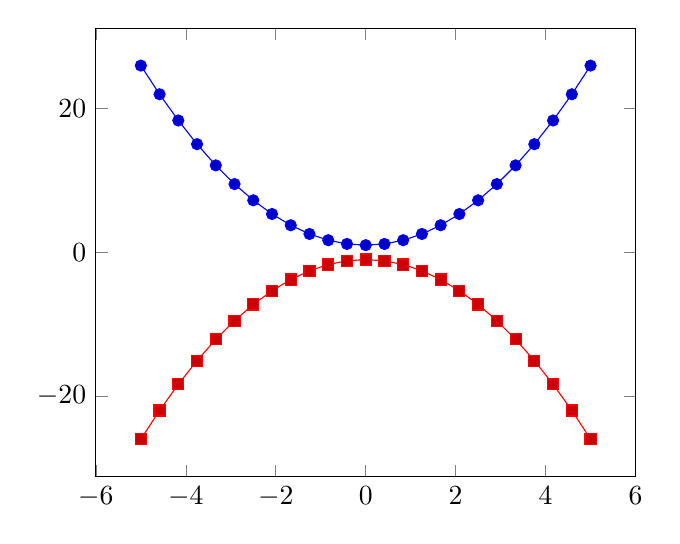
\begin{tikzpicture}
\begin{axis}
\addplot {x^2+1};
\addplot {-x^2-1};
\end{axis}
\end{tikzpicture}

\end{eg}

\begin{notation}
$B_\varepsilon^k = B_\varepsilon\left(\mathbf{0}\right) \subset \R^k$ = $k-$dimensional open ball.
\end{notation}

\begin{thm}
Suppose $F:\R^n \to \R^m$ is $C^1$, $f\left(\mathbf{x}_0\right) = \mathbf{y}_0$, and $DF|_{\mathbf{x}_0}$ is surjective. Then there's an open set $V \subset \R^n$, $\mathbf{x}_0 \in V$, and a $C^1$ map $G: B_\varepsilon^{n-m} \to \R^n$ such that:\\
1) $F^{-1} \left(\mathbf{y}_0\right) \cap V = \im G$;\\
2) $G$ is injective;\\
3) $DG|_\mathbf{z}$ is injective for all $\mathbf{z} \in B_\varepsilon^{n-m}$.\\
i.e. if $n-m=1$, $B'_\varepsilon = \left(-\varepsilon,\varepsilon\right)$, $F^{-1}\left(\mathbf{y}_0\right) \cap V$ is a paramterized curve;\\
if $n-m = 2$ then this is a parametrized surface.\\
For general $n-m$, we call this is a parametrized $(n-m)$-manifold.
\end{thm}

\begin{eg}
$F\left(x,y\right) = x^2-y^2$, $DF|_{(x,y)} = \left[2x,-2y\right]$ is surjective $\iff$ $\left(x,y\right) \neq \left(0,0\right)$.
\end{eg}

\begin{defi}
$F^{-1}\left(\mathbf{y}_0\right)$ is \emph{smooth} at $\mathbf{x}_0$ if $DF|_{\mathbf{x}_0}$ is surjective, \emph{singular} at $\mathbf{x}_0$ otherwise.\\
$F^{-1}\left(\mathbf{y}_0\right)$ is smooth if it is smooth at all $\mathbf{x} \in F^{-1} \left(\mathbf{y}_0\right)$.
\end{defi}

Proof of theorem:
\begin{proof}
$DF|_{\mathbf{x}_0}: \R^n \to \R^m$ is surjective. So $K := \ker DF|_{\mathbf{x}_0}$ has dimension $(n-m)$. Choose any $\pi \in \mathcal{L}\left(\R^n,\R^m\right)$ with $\pi\left(K\right) = \R^{n-m}$. Define $f: \R^n \to \R^m \times \R^{n-m} = \R^n$ by $f\left(\mathbf{x}\right) = \left(F\left(\mathbf{x}\right),\pi\left(\mathbf{x}\right)\right)$. So $Df:\R^n \to \R^m \oplus \R^{n-m}$.\\
$Df_{\mathbf{x}_0} \left(\mathbf{v}\right) = \left(DF|_{\mathbf{x}_0} \left(\mathbf{v}\right), \pi\left(\mathbf{v}\right)\right)$ since $D\pi = \pi$.\\
Claim: $Df|_{\mathbf{x}_0}$ is an isomorphism: If $Df|_{\mathbf{x}_0} \left(\mathbf{v}\right) = \mathbf{0}$, then $DF|_{\mathbf{x}_0} \left(\mathbf{v}\right) = 0 \implies \mathbf{v} \in K$. But $\pi: K \to \R^{n-m}$ is an isomorphism, so $\pi\left(\mathbf{v}\right) = 0 \implies \mathbf{v} = 0$. So $\ker Df|_{\mathbf{x}_0} = \left\{\mathbf{0}\right\}$ $\implies$ $Df|_{\mathbf{x}_0}$ is an isomorphism.

By the inverse function theorem, there exists $V \subset \R^n$, $\mathbf{x}_0 \in V$, $W \subset \R^m \times \R^{n-m}$, $\left(\mathbf{y}_0,\pi\left(\mathbf{x}_0\right)\right) \in W$, s.t. $f:V \to W$ is an diffeomorphism. Let $g = f^{-1} : W \to V$

Then $F^{-1}\left(\mathbf{y}_0\right) \cap V = f^{-1} \left(\mathbf{y}_0 \times \R^{n-m}\right) \cap V$, so $g\left(\mathbf{y}_0 \times \R^{n-m} \right) \cap W = F^{-1}\left(\mathbf{y}_0\right) \cap V$.

Define $G\left(\mathbf{z}\right) = g\left(\mathbf{y}_0,\mathbf{z}_0\right)$, $g$ is injective implies that $G$ is injective, and $D_g$ injective $\implies$ $DG$ injective.
\end{proof}

\end{document}